% ch08a Quenching of local moments: the Kondo problem, part a (书页 80-101 / 分册p001-022)
% 第8章 Quenching of local moments: the Kondo problem
\chapter{局域磁矩的淬灭：近藤问题}

上一章中，我们针对金属中局域磁矩（local moment）的形成建立了一个平均场判据。由于平均场理论通常只在高温下有效，我们预期在低温下这一处理会出现显著的偏离。本章关注的两个问题是：（1）局域磁矩的存在如何影响宿主金属的低温输运性质与磁性；（2）金属中的局域磁矩在低温下的命运究竟如何？这些问题具有极其重要的实验意义，因为早在20世纪30年代初人们就已经知道，像Cu这样含有痕量磁性杂质（典型为Fe）的宿主金属，其电阻率会达到一个极小值，随后随温度继续降低而按$-\ln T$增大。各种Mo与Nb合金的这种行为示于图 8.1（SCL1964）。电阻率极小及其后的对数式温度依赖，与纯金属的电阻率形成鲜明对比——后者随温度降低单调地趋于零。另一个令人意外的事实是，电阻率的$-\ln T$依赖并不会无限延续到低温，而是在低于某一特征温度——近藤温度（Kondo temperature）$T_{\mathrm{k}}$——之后逐渐消退。此外，磁化率测量（H1969）表明，磁性杂质的自旋性质在近藤温度附近发生根本的改变。远高于近藤温度时，杂质自旋的磁化率服从自由磁矩的居里$1/T$定律；而低于$T_{\mathrm{k}}$时，磁化率趋于一个常数（H1969）。$T=0$处的常数磁化率正是被磁场极化的单态的特征（习题8.1）。因此，$T_{\mathrm{k}}$除了是电阻率的$-\ln T$行为终止的温度之外，还是杂质自旋与传导电子自旋开始凝聚成单态的温度。这一凝聚在$T=0$时进行完全。局域磁矩在某一特征温度以下消失，这使得近藤问题与体铁磁性有着本质的不同——在体铁磁性中，磁性是在某一特征温度（居里温度）以下开始出现的。近藤问题恰恰相反：磁性在低温下终止。

既然杂质一旦开始凝聚成单态，电阻率的$-\ln T$依赖便随之消失，电阻率极小就必定源于杂质自旋与宿主金属自旋之间的相互作用。最早能够描述局域自旋与巡游传导电子相互作用的模型，发端于20世纪40年代与50年代Vousovskii（V1946）、齐纳（Zener，Z1951）和笠谷（Kasuya，K1956）的工作。该模型的要点是：局域杂质自旋与传导电子之间存在交换相互作用（exchange interaction）$J$。正如我们将要证明的，这一模型在一定参数范围内与安德森（Anderson）模型相关联。

\begin{figure}[H]\centering
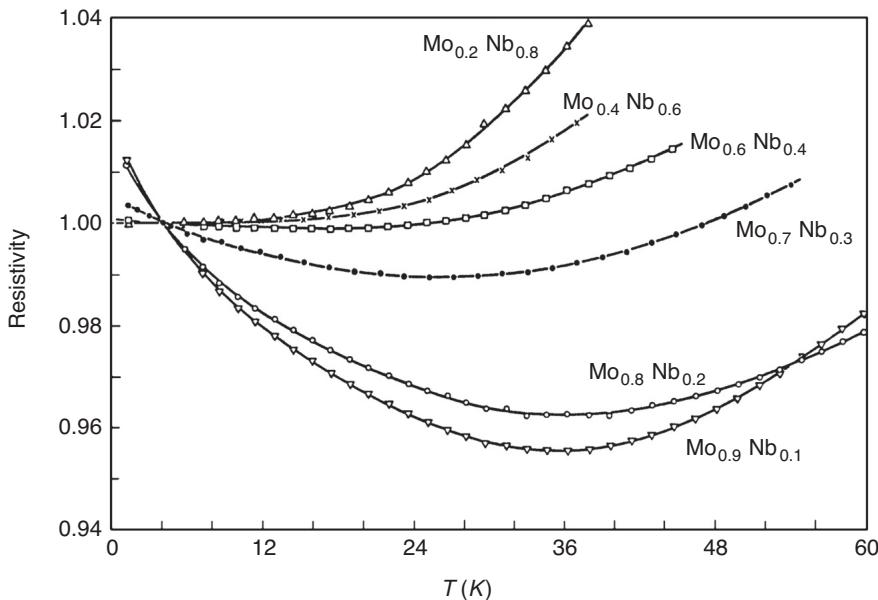
\includegraphics[width=0.62\textwidth]{figs/ch08/fig_8.1.jpg}
\caption*{图 8.1\quad 一系列Mo–Nb合金中Fe的电阻极小（取自Sarachik et al., Phys. Rev. 135, 1041 (1964)）。}\label{fig:auto:8.1}
\end{figure}

近藤证明，在按$J$展开到二阶的微扰论中会出现一个$-\ln T$项。除了低温下按$T^5$标度的传导电子–声子散射率之外，这类散射过程也对散射率有贡献。由于电阻率正比于总散射概率，自旋翻转散射带来的对数贡献意味着电阻率中会出现一个极小。近藤的微扰处理由此为金属合金中电阻率极小这一长期悬而未决的问题提供了解答。

然而，近藤的解答并非完美无缺。当$T\to 0$时，$\ln T$项发散。在散射概率的微扰处理中，二阶项在量级上变得可与一阶项相比时的温度，决定了发散何时发生。这一温度称为$T_{\mathrm{k}}$，系统的磁学性质正是在这一温度附近发生改变。发散意味着微扰论在低温下失效。因此，近藤的解答只在$T\gg T_{\mathrm{k}}$时有效；要理解磁性杂质在$T_{\mathrm{k}}$附近及其以下的最终命运，必须发展别的方法。不过实验告诉我们，局域磁矩最终在$T=0$时是不能存活的。为消除近藤微扰处理中的发散、并解释杂质处束缚单态（bound singlet state）的形成而寻找理论的努力，被称为“近藤问题”。

安德森等人（AYH1970）的标度假设（scaling hypothesis）是通往这一相当微妙问题之解答的关键概念。他们在微扰框架内证明，随着把越来越多高能激发对有效积分的影响包括进来，近藤问题中交换相互作用的数值不断增大。他们的方案虽属微扰性质，却对准确指认局域矩消失、基态单态随之形成的物理机制起了关键作用。不过，这一问题的关键突破发生在20世纪70年代后期，当时威尔逊（Wilson，W1975）发展了数值重正化群方法来求解近藤问题。他的解证实了安德森与Yuval的标度假设。近藤问题的解决居然需要动用现代理论物理的关键思想之一，这一点当初完全没有被预料到。的确，近藤模型的简单性掩盖了它所体现的物理的复杂性。部分正因如此，在电阻率极小得到满意解释之后很久，束缚单态的起源仍然被笼罩在发散的微扰求和之中。

本章中，我们将给出导致电阻率极小问题和近藤问题得以解决的关键思想。我们首先给出近藤模型，并确立局域磁矩与传导电子之间反铁磁相互作用的起源。在此过程中我们将能厘清安德森模型与近藤模型之间的关系。有了反铁磁相互作用，我们随后进行二阶微扰分析，以揭示电阻率中的$\ln T$依赖。将会看到：只要局域杂质具有某种自由度（对局域磁矩而言即自旋），电导率就会出现$\ln T$依赖。最后我们讨论束缚单态形成的变分分析与标度分析。

\section{近藤哈密顿量}

近藤哈密顿量描述杂质自旋（假定其为自旋$1/2$）与传导电子自旋之间的相互作用。我们先引入从杂质态和传导态中移除电子的二分量旋量算符：
\begin{equation*}
\Psi_{\mathbf{k}} = \begin{pmatrix} a_{\mathbf{k}\uparrow} \\ a_{\mathbf{k}\downarrow} \end{pmatrix}, \quad \Psi_d = \begin{pmatrix} a_{d\uparrow} \\ a_{d\downarrow} \end{pmatrix}
\tag{8.1}
\end{equation*}
以及自旋矩阵算符
\begin{equation*}
\mathbf{S} = \frac{\hbar\sigma}{2},
\tag{8.2}
\end{equation*}
其中$\sigma$是通常的泡利矩阵，
\begin{equation*}
\sigma_x = \begin{pmatrix} 0 & 1 \\ 1 & 0 \end{pmatrix}, \quad \sigma_y = \begin{pmatrix} 0 & -\mathrm{i} \\ \mathrm{i} & 0 \end{pmatrix}, \quad \sigma_z = \begin{pmatrix} 1 & 0 \\ 0 & -1 \end{pmatrix}.
\tag{8.3}
\end{equation*}
我们还将用到自旋升算符$\hbar\sigma^+/2 = S_x + \mathrm{i}S_y = S^+$与自旋降算符$\hbar\sigma^-/2 = S_x - \mathrm{i}S_y = S^-$。

近藤物理源于杂质自旋与传导电子自旋的耦合。于是，表示局域自旋与一团巡游电子相互作用的最简单的哈密顿量为
\begin{equation*}
H_{\mathrm{K}} = \sum_{\mathbf{k},\sigma}\epsilon_{\mathbf{k}} n_{\mathbf{k}\sigma} - \sum_{\mathbf{k},\mathbf{k}'}\frac{J_{\mathbf{k}\mathbf{k}'}}{\hbar^2}\left(\Psi_{\mathbf{k}'}^{\dagger}\mathbf{S}\Psi_{\mathbf{k}}\right)\cdot\left(\Psi_d^{\dagger}\mathbf{S}\Psi_d\right).
\tag{8.4}
\end{equation*}
算符$\Psi_d^{\dagger}\mathbf{S}\Psi_d$是杂质态$d$中电子的自旋算符，而自旋算符$\Psi_{\mathbf{k}'}^{\dagger}\mathbf{S}\Psi_{\mathbf{k}}$则是电子在传导态$\mathbf{k}$与$\mathbf{k}'$之间的\emph{跃迁}自旋算符。由于局域杂质能量仅仅移动能量的零点，我们已把这一项从哈密顿量中略去。相互作用$J_{\mathbf{k}\mathbf{k}'}$具有能量量纲，它是带电子自旋与局域电子自旋之间海森堡自旋交换相互作用的类似物。正的$J_{\mathbf{k}\mathbf{k}'}>0$倾向于自旋平行排列（见第5章式 (5.18)），因而描述铁磁相互作用；而$J_{\mathbf{k}\mathbf{k}'}<0$对应于反铁磁相互作用。

\section{为何$J$是负的？}

本节我们为近藤哈密顿量中的交换相互作用给出一个简单的物理推导，所依据的是安德森的磁性杂质模型。完整的推导详见本章附录。近藤问题中的相互作用只有在杂质上存在净自旋时才不为零——对一个至多可被双占据的杂质而言，即处于局域矩相时。正如上一章所讨论的，安德森模型中的局域矩相持续存在于在位库仑相互作用$U$远大于杂化能$\Delta$的极限。正是在局域矩极限下，安德森模型与近藤模型描述相同的物理。然而，安德森模型与近藤模型的一个根本差别在于：安德森模型包含电荷涨落——正是电荷涨落决定了杂化能——而近藤模型只包含自旋–自旋相互作用，不含电荷涨落。正如我们现在要证明的，把电荷涨落算到杂化矩阵元$V_{\mathbf{k}d}$的二阶，其效应会导致近藤模型中那一类型的反铁磁相互作用。

我们聚焦于安德森模型中导致传导电子被局域矩散射的那些过程，并对使传导电子与局域矩相耦合的杂化相互作用$\propto V_{\mathbf{k}d}$计算到二阶。在微扰论中，这类过程的振幅具有如下形式
\begin{equation*}
V_{\mathbf{k}d}\frac{1}{E_{\mathrm{i}}-E_{\mathrm{int}}}V_{d\mathbf{k}},
\tag{8.5}
\end{equation*}
其中$E_{\mathrm{i}}$是初态能量，$E_{\mathrm{int}}$是中间态能量。我们先考虑态$\mathbf{k}$中自旋向下的传导电子被自旋向上的杂质散射、到达自旋向下的终态电子态$\mathbf{k}'$且杂质保持自旋向上的过程。如图 8.2(a)所示，这一过程通过电子$\mathbf{k}$经杂化相互作用跳跃到杂质上而发生；在此中间态中，杂质被双占据。中间态的能量为$2\epsilon_d+U$。随后，杂质上的下自旋电子再跳跃到终态传导电子态$\mathbf{k}'$。该过程的二阶矩阵元为
\begin{equation*}
T_{(\mathbf{k}\sigma)+(d-\sigma)\to(\mathbf{k}'\sigma)+(d-\sigma)} = \frac{V_{\mathbf{k}d}V_{d\mathbf{k}'}}{\epsilon_{\mathbf{k}}-\epsilon_d-U}.
\tag{8.6}
\end{equation*}

\begin{figure}[H]\centering
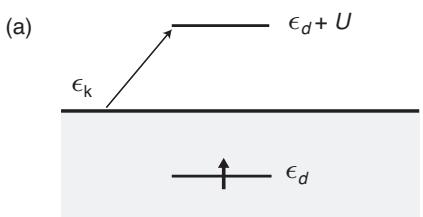
\includegraphics[width=0.5\textwidth]{figs/ch08/fig_8.2_a.jpg}\\[6pt]
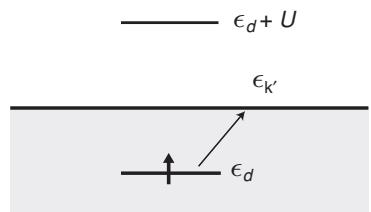
\includegraphics[width=0.5\textwidth]{figs/ch08/fig_8.2_b.jpg}
\caption*{图 8.2\quad 对单占据d能级的二阶电荷涨落有贡献的两个过程。实线表示恰在费米面之下的初始传导电子态。能级的标注方式与第7章相同。}\label{fig:auto:8.2}
\end{figure}

另一方面，态$\mathbf{k}$中自旋向上的传导电子与自旋向上杂质的散射——到达自旋向上的终态电子态$\mathbf{k}'$且杂质保持自旋向上——只能经由杂质上的电子先跳跃到$\mathbf{k}'$来进行，如图 8.2(b)所示。在中间态，两个电子都处于传导态。矩阵元于是为
\begin{equation*}
T_{(\mathbf{k}\sigma)+(d\sigma)\to(\mathbf{k}'\sigma)+(d\sigma)} = -\frac{V_{\mathbf{k}d}V_{d\mathbf{k}'}}{\epsilon_d-\epsilon_{\mathbf{k}'}}.
\tag{8.7}
\end{equation*}
负号来自传导电子与杂质电子的交换；初始的传导电子终于杂质之上，而杂质上最初的电子则进入导带。类似地，态$\mathbf{k}$中自旋向上电子与自旋向下杂质之间的自旋翻转散射——终态电子为$\mathbf{k}'\downarrow$、杂质最终自旋向上——既可以经由这一同样的过程进行，也可以按如下方式进行：一个传导电子先跳跃到杂质上，然后杂质上的下自旋电子再跳跃到终态$\mathbf{k}'$。振幅是各单个过程振幅的线性叠加：
\begin{equation*}
T_{(\mathbf{k}\sigma)+(d-\sigma)\to(\mathbf{k}'-\sigma)+(d\sigma)} = -V_{\mathbf{k}d}V_{d\mathbf{k}'}\left(\frac{1}{\epsilon_{\mathbf{k}}-\epsilon_d-U}+\frac{1}{\epsilon_d-\epsilon_{\mathbf{k}'}}\right).
\tag{8.8}
\end{equation*}
负号同样来自传导电子与杂质电子的交换。

如附录所示，近藤模型的自旋–自旋相互作用式 (8.4) 给出自旋翻转过程的振幅
\begin{equation*}
T_{(\mathbf{k}\sigma)+(d-\sigma)\to(\mathbf{k}'-\sigma)+(d\sigma)} = -\frac{1}{2}J_{\mathbf{k}\mathbf{k}'}.
\tag{8.9}
\end{equation*}
于是，从式 (8.8) 与式 (8.9) 我们推得
\begin{equation*}
J_{\mathbf{k}\mathbf{k}'} = 2V_{\mathbf{k}d}V_{d\mathbf{k}'}\left(\frac{1}{\epsilon_{\mathbf{k}}-\epsilon_d-U}+\frac{1}{\epsilon_d-\epsilon_{\mathbf{k}'}}\right).
\tag{8.10}
\end{equation*}

若假定宿主金属中相关的$\mathbf{k}$态都靠近费米能级，即$\epsilon_{\mathbf{k}}\approx\epsilon_{\mathbf{k}'}\approx 0$，则此表达式化为
\begin{equation*}
J_{\mathrm{eff}} = -|V_{\mathbf{k}d}|^2\frac{U}{|\epsilon_d|(U-|\epsilon_d|)} < 0.
\tag{8.11}
\end{equation*}

d杂质与电子带之间的有效耦合确实是反铁磁的。为确定其大小，我们考虑$\epsilon_d=-U/2$的粒子–空穴对称点。在此极限下，交换相互作用
\begin{equation*}
J_{\mathrm{eff}} = -4\frac{|V_{\mathbf{k}d}|^2}{U},
\tag{8.12}
\end{equation*}
与在位库仑排斥成反比。在安德森模型中，导带与杂质之间的电荷涨落传递了近藤相互作用。安德森哈密顿量在近藤极限下的耦合常数按$\Delta/U\ll 1$标度。我们在这里导出的相互作用是按$V_{\mathbf{k}d}$展开的微扰级数中最低阶的一项。为什么把电荷涨落考虑到二阶会导致相互作用依赖自旋？物理上的答案是泡利不相容原理：它禁止杂质被两个自旋取向相同的电子占据的中间态。

在本章附录中，我们经由Schrieffer–Wolff变换导出精确到$V_{\mathbf{k}d}$二阶的完整哈密顿量。$J_{\mathbf{k}\mathbf{k}'}$与式 (8.10) 的唯一差别在于，完整的结果式 (8.122) 对两个波矢$\mathbf{k}$与$\mathbf{k}'$是对称化的。读者应当自行验证：式 (8.7) 中等自旋过程的完整振幅来自直接相互作用$H_{\mathrm{dir}}$（式 (8.125)），而式 (8.6) 中相反自旋过程的完整振幅则同时来自直接相互作用与自旋–自旋相互作用。

近藤模型在局域矩相中与安德森模型的等价，暗示两个模型的基态应当相同。天真地，人们会把安德森模型中单态的形成与杂质能级的双占据联系起来。这一诠释是有问题的，因为在安德森模型的局域矩相中，上能级并未被占据。此外，当温度降低时，杂质能级相对费米能级的位置保持不变，上能级（能量为$\epsilon_d+U$）仍远高于费米能级。因此它必定是空的，如图 8.3所示。

\begin{figure}[H]\centering
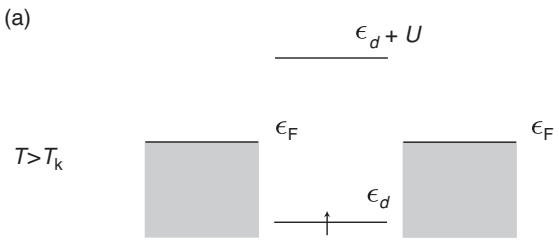
\includegraphics[width=0.5\textwidth]{figs/ch08/fig_8.3_a.jpg}\\[6pt]
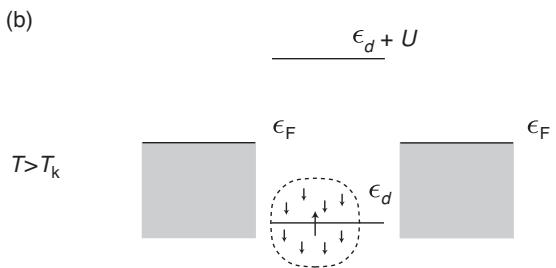
\includegraphics[width=0.5\textwidth]{figs/ch08/fig_8.3_b.jpg}
\caption*{图 8.3\quad 安德森模型中能级的示意图：(a) 高于近藤温度时；(b) 低于近藤温度时。尽管当温度降到$T_{\mathrm{k}}$以下时局域矩开始消失，上能级的占据数却保持为零、毫无变化。这一奇怪的情形正是近藤问题。注意，费米海在近藤温度以下并不产生净磁化。}\label{fig:auto:8.3}
\end{figure}

理解安德森模型在$T=0$时单态基态的起源，正是近藤问题的实质。单态的出现是一个新的共振能级（resonant level）（GZ1972）形成并钉扎在费米能级处的结果。共振能级的形成所致安德森模型单粒子态密度的改变示于图 8.4。峰随温度降低对数式地增长（L1981），直至近藤温度；其宽度正比于$T_{\mathrm{k}}$。总的说来，能量处于费米面附近$T_{\mathrm{k}}$范围内的所有传导电子都对共振能级的形成有贡献，如图 8.3所绘。对自旋$1/2$的杂质，共振能级平均只被一个传导电子占据，该电子抵消了杂质上的自旋。正如我们在8.4节末尾将要讨论的，正是电子–杂质散射率中的对数奇异性产生了费米能级处单粒子态密度的尖峰。费米能级处超额的态密度随杂质自旋的消失而增长。

总而言之，在高温下局域磁矩形成的哈特里–福克理论有效，杂质态密度由上一章导出的双峰洛伦兹函数很好地描述。然而在低温下，出现了安德森模型平均场描述无法刻画的新物理。低温下，传导电子与局域磁矩之间发生快速的自旋翻转散射。下面我们就来说明这类过程如何构成金属合金中电阻率极小的根源。

\begin{figure}[H]\centering
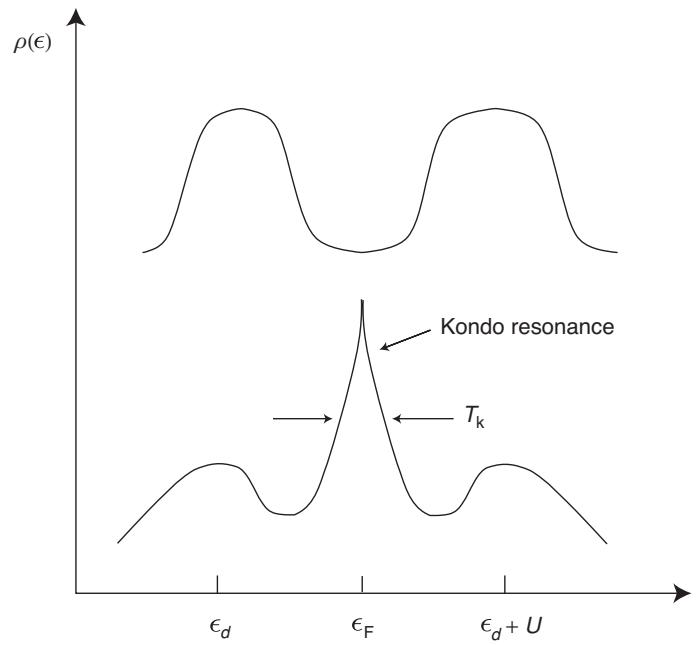
\includegraphics[width=0.55\textwidth]{figs/ch08/fig_8.4.jpg}
\caption*{图 8.4\quad 近藤区间内安德森模型的单粒子态密度。费米能级处尖峰的出现是一种多体共振效应。随着温度降低，此峰对数式地增大。}\label{fig:auto:8.4}
\end{figure}

\section{散射与电阻率极小}

电阻率中对数贡献的起源是杂质处的自旋自由度。为看清自旋的作用，我们概述散射概率结构所依赖的关键概念。我们将会看到，准确到交换相互作用最低阶的散射概率行为良好且与温度无关。温度依赖首先出现在把散射振幅计算到交换相互作用二阶时。由于相互作用依赖自旋自由度，二阶项可以涉及杂质上的自旋翻转过程。然而，自旋翻转的先后次序是重要的，例如$S^+S^-\neq S^-S^+$。这种不可对易性，加上泡利原理对中间态允许占据方式的限制，导致散射振幅出现非平庸的温度依赖。二阶贡献形如$f/\epsilon$。这一积分对数式发散，这就是近藤对数（Kondo logarithm）的起源。相反，若杂质没有任何内部结构，泡利原理对中间态填充的限制将完全相消。

现在我们来补足把散射振幅计算到交换相互作用二阶的推导细节。由于交换相互作用是短程的点状相互作用，其傅里叶变换在$k$空间应为常数。于是我们作近似
\begin{equation*}
J_{\mathbf{k}\mathbf{k}'} = J_0/V,
\tag{8.13}
\end{equation*}
其中$J_0$是负的常数，$V$是体积。近藤哈密顿量是一个未微扰部分
\begin{equation*}
H_0 = \sum_{\mathbf{k},\sigma}\epsilon_{\mathbf{k}} n_{\mathbf{k}\sigma}
\tag{8.14}
\end{equation*}
与自旋–自旋相互作用之和，后者按微扰处理：
\begin{equation*}
H' = -\frac{J_0}{2\hbar V}\sum_{\mathbf{k}',\mathbf{k}''}\left[S_d^z\left(a_{\mathbf{k}'\uparrow}^{\dagger}a_{\mathbf{k}''\uparrow}-a_{\mathbf{k}'\downarrow}^{\dagger}a_{\mathbf{k}''\downarrow}\right)+S_d^{+}a_{\mathbf{k}'\downarrow}^{\dagger}a_{\mathbf{k}''\uparrow}+S_d^{-}a_{\mathbf{k}'\uparrow}^{\dagger}a_{\mathbf{k}''\downarrow}\right].
\tag{8.15}
\end{equation*}
由于我们只关心与单个杂质的耦合，这里用单个杂质自旋算符$\mathbf{S}_d$来写这一相互作用，而不是用近藤哈密顿量（式 (8.4)）中对杂质的二次量子化描述。为练习自旋代数，我们更一般地假定杂质总自旋为$S\equiv\hbar s$；$S_z$的本征态用本征值$\hbar m_{\mathrm{s}}$标记。

我们先以最低阶计算杂质把初始动量为$\mathbf{k}$的传导电子散射到动量$\mathbf{k}'$的总速率；设杂质的初始自旋取向为$m_{\mathrm{s}}$。多粒子电子态是导带中单粒子态的斯莱特行列式。由于$H'$只含导带的一对产生和湮灭算符，它只能连接相差单个轨道的态。因此，进入散射速率计算的能量差化为单轨道能量之差。

总散射速率是两个非相干过程速率之和：第一个过程中初始电子（取为自旋向上）不翻转自旋并保持自旋向上；第二个过程中电子从自旋向上变到自旋向下，而杂质从$m_{\mathrm{s}}$变到$m_{\mathrm{s}}+1$。先考虑非自旋翻转过程，其裸矩阵元为
\begin{equation*}
T_{\mathbf{k}\uparrow\to\mathbf{k}'\uparrow;m_{\mathrm{s}}}^{(0)} = -\frac{J_0}{2V}m_{\mathrm{s}}.
\tag{8.16}
\end{equation*}
最低阶散射速率为
\begin{equation*}
\Gamma_{\mathbf{k}\to\mathbf{k}'}^{0}(m_{\mathrm{s}}) = \frac{2\pi}{\hbar}\sum_{\mathbf{k}'}\delta(\epsilon_{\mathbf{k}}-\epsilon_{\mathbf{k}'})\left(\frac{J_0}{2V}\right)^2 m_{\mathrm{s}}^2,
\tag{8.17}
\end{equation*}
其中求和遍及有限的一组终态$\mathbf{k}'$。注意散射是各向同性的（$s$波）。为计算这一过程的总速率，我们把$\mathbf{k}'$对所有终态求和，当$\mathbf{k}$靠近费米面时给出因子$N(0)V$，其中$N(0)=mk_{\mathrm{F}}/2\pi^2\hbar^2=3n_{\mathrm{e}}/4\epsilon_{\mathrm{F}}$是费米面处单自旋电子态密度。于是，单个杂质无非自旋翻转的总散射速率为
\begin{equation*}
\Gamma_{\mathrm{non\text{-}flip}}^{0}(m_{\mathrm{s}}) = \frac{\pi}{2\hbar V}N(0)J_0^2 m_{\mathrm{s}}^2.
\tag{8.18}
\end{equation*}
在自旋翻转过程中，矩阵元为
\begin{equation*}
T_{\mathbf{k}\uparrow\to\mathbf{k}'\downarrow;m_{\mathrm{s}}}^{(0)} = -\frac{J_0}{2\hbar V}\langle s,m_{\mathrm{s}}+1|S_d^{+}|s,m_{\mathrm{s}}\rangle.
\tag{8.19}
\end{equation*}
由角动量的量子理论，
\begin{equation*}
\langle s,m_{\mathrm{s}}\pm 1|S^{\pm}|s,m_{\mathrm{s}}\rangle = \hbar\sqrt{s(s+1)-m_{\mathrm{s}}(m_{\mathrm{s}}\pm 1)},
\tag{8.20}
\end{equation*}
于是
\begin{equation*}
\Gamma_{\mathrm{flip}}^{0}(m_{\mathrm{s}}) = \frac{\pi}{2\hbar V}N(0)J_0^2\left(s(s+1)-m_{\mathrm{s}}(m_{\mathrm{s}}+1)\right).
\tag{8.21}
\end{equation*}
总散射速率为式 (8.18) 与式 (8.21) 之和：
\begin{equation*}
\Gamma^{0}(m_{\mathrm{s}}) = \frac{\pi}{2\hbar V}N(0)J_0^2\left(s(s+1)-m_{\mathrm{s}}\right).
\tag{8.22}
\end{equation*}
若对杂质所有初始自旋取向平均，$m_{\mathrm{s}}$项消失。再对所有杂质求和，我们得到自旋平均后的散射速率
\begin{equation*}
\Gamma^{0} = \frac{\pi}{2\hbar}s(s+1)J_0^2 n_{\mathrm{imp}}N(0) = \frac{2\pi}{3}\frac{\epsilon_{\mathrm{F}}}{\hbar}s(s+1)c(N(0)J_0)^2,
\tag{8.23}
\end{equation*}
其中$c=n_{\mathrm{imp}}/n_{\mathrm{e}}$是分数浓度（fractional concentration），$n_{\mathrm{imp}}$是杂质密度。非自旋翻转贡献占总量的$1/3$，这可从关系式
\begin{equation*}
\frac{1}{2s+1}\sum_{m_{\mathrm{s}}}m_{\mathrm{s}}^2 = \frac{1}{3}s(s+1).
\tag{8.24}
\end{equation*}
看出。

散射速率式 (8.23) 行为良好且完全与温度无关。若一切条件相同，微扰论每高一级就小一个因子$J_0N(0)$。如此看来似乎没有必要去探究二阶项。然而条件并不相同，一个关键的发散正潜伏在二阶。

为确定下一阶的散射速率，我们把散射振幅计算到二阶。一般地，二阶振幅由下式给出：
\begin{equation*}
T_{a\to b}^{(2)} = \sum_{c\neq a}\frac{\langle b|H'|c\rangle\langle c|H'|a\rangle}{E_a-E_c}.
\tag{8.25}
\end{equation*}

与最低阶时一样，散射速率是如下两类过程之和：初、末电子态自旋相同的过程，以及末态电子自旋与初态相反的过程。图 8.5 显示了末态电子与初态自旋相同时振幅的二阶贡献，图 8.6 显示了末态自旋发生翻转的过程。在每一过程中，进入中间态的贡献有两类：非自旋翻转项——电子自旋保持不变且只涉及$S^z$——以及涉及算符$S^{\pm}$的自旋翻转项。

\begin{figure}[H]\centering
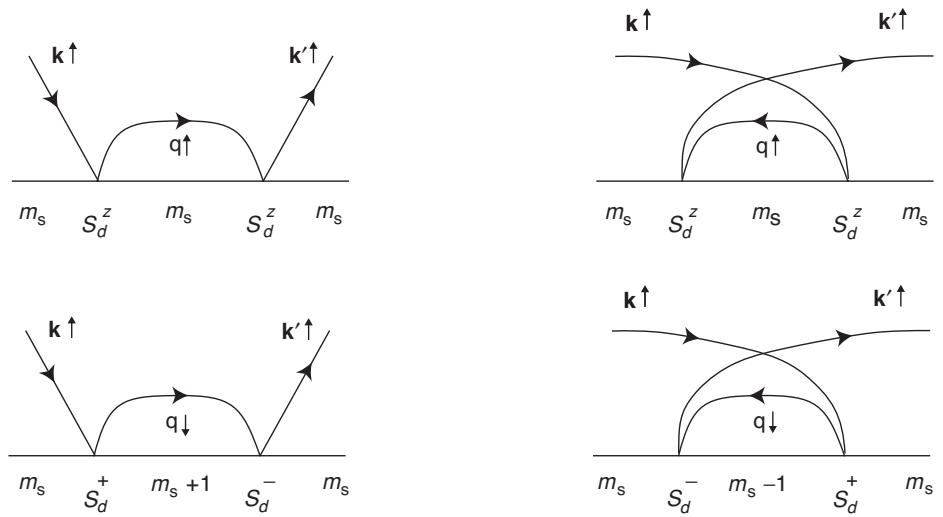
\includegraphics[width=0.72\textwidth]{figs/ch08/fig_8.5.jpg}
\caption*{图 8.5\quad 初、末电子态为$\mathbf{k}\uparrow$与$\mathbf{k}'\uparrow$的二阶过程。直线描绘杂质自旋，曲线描绘电子。中间态中带反向箭头的线代表空穴，即一个在初态和末态都存在、但在中间态缺席的粒子。空穴上的标记是该电子在初态中的动量与自旋。}\label{fig:auto:8.5}
\end{figure}

\begin{figure}[H]\centering
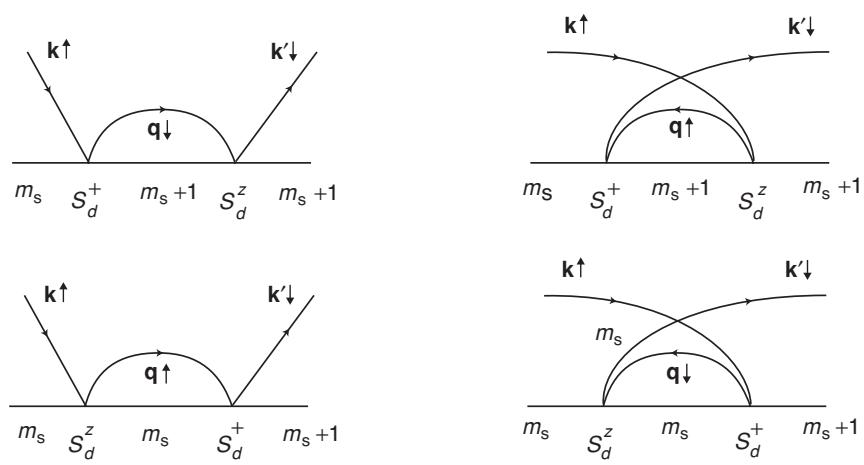
\includegraphics[width=0.72\textwidth]{figs/ch08/fig_8.6.jpg}
\caption*{图 8.6\quad 初、末电子态为$\mathbf{k}\uparrow$与$\mathbf{k}'\downarrow$的二阶自旋翻转过程。}\label{fig:auto:8.6}
\end{figure}

我们先考虑图 8.5 中上面的两个过程，其中初始动量为$\mathbf{k}$的电子被散射到末动量$\mathbf{k}'$。一方面，电子可以从动量$\mathbf{k}$散射到一个动量为$\mathbf{q}$的未占据态，随后再到达动量为$\mathbf{k}'$的终态，如左上图所示。这一过程对$T_{\mathrm{non\text{-}flip}}^{(2)}(\mathbf{k}\to\mathbf{k}';m_{\mathrm{s}})$的贡献为
\begin{equation*}
\left(\frac{-J_0 m_{\mathrm{s}}}{2}\right)^2\frac{1}{V}\alpha,
\tag{8.26}
\end{equation*}
其中对中间粒子态的求和为
\begin{equation*}
\alpha = \frac{1}{V}\sum_{\mathbf{q}}\frac{1-f_{\mathbf{q}}}{\epsilon_{\mathbf{k}}+\mathrm{i}\eta-\epsilon_{\mathbf{q}}}.
\tag{8.27}
\end{equation*}
因子$1-f_{\mathbf{q}}$（$f_{\mathbf{q}}$为电子的费米分布函数）保证态$\mathbf{q}$是空的。正的无穷小虚数$\mathrm{i}\eta$保证散射产生的是出射波而非入射波。在量子力学上与该过程相干的是右上图（见图 8.5）所示的过程：处于占据态$\mathbf{q}$的一个电子散射到终态$\mathbf{k}'$，而另一个动量为$\mathbf{k}$的电子则散射进入腾出来的态$\mathbf{q}$，其贡献为
\begin{equation*}
\left(\frac{-J_0 m_{\mathrm{s}}}{2V}\right)^2\frac{1}{V}\gamma,
\tag{8.28}
\end{equation*}
其中
\begin{equation*}
\gamma = -\frac{1}{V}\sum_{\mathbf{q}}\frac{f_{\mathbf{q}}}{\epsilon_{\mathbf{q}}+\mathrm{i}\eta-\epsilon_{\mathbf{k}'}}.
\tag{8.29}
\end{equation*}
在后一过程中，中间动量态必须被占据，故速率正比于$f_{\mathbf{q}}$。负号来自移除初始电子与产生终态电子这两个操作的交换：当$\mathbf{k}\neq\mathbf{k}'$时$a_{\mathbf{k}}a_{\mathbf{k}'}^{\dagger}=-a_{\mathbf{k}'}^{\dagger}a_{\mathbf{k}}$。在能量守恒的散射（$\epsilon_k=\epsilon_{k'}$）过程中，两个过程的振幅相加时分布函数相消，非自旋翻转过程的振幅为
\begin{equation*}
T_{\mathrm{non\text{-}flip}}^{(2)}(\mathbf{k}\uparrow\to\mathbf{k}'\uparrow;m_{\mathrm{s}}) = \left(\frac{-J_0 m_{\mathrm{s}}}{2V}\right)^2\sum_{\mathbf{q}}\frac{1}{\epsilon_{\mathbf{k}}-\epsilon_{\mathbf{q}}}.
\tag{8.30}
\end{equation*}
由于诸$f$相消，非自旋翻转振幅与温度无关。这一求和形式上发散，因为我们忽略了矩阵元的动量依赖；一旦把它考虑进来，该项便是有限的。

图 8.5 中下面的两个过程在中间态涉及一次电子自旋翻转。与上面讨论的非自旋翻转过程一样，进入的也是同样两个中间动量态；但两者的权重不同。在左下图中，矩阵元给出因子 $(-J_0/2\hbar V)^{2}P_{+-}$，其中
\begin{equation*}
P_{+-} = \frac{1}{\hbar^2}\left|\langle s,m_{\mathrm{s}}+1|S_d^{+}|s,m_{\mathrm{s}}\rangle\right|^2 = s(s+1)-m_{\mathrm{s}}(m_{\mathrm{s}}+1).
\tag{8.31}
\end{equation*}
在右下图中，中间态涉及一个被填充的态，矩阵元给出的则是$(-J_0/2\hbar V)^2P_{-+}$，其中
\begin{equation*}
P_{-+} = \frac{1}{\hbar^2}\left|\langle s,m_{\mathrm{s}}-1|S_d^{-}|s,m_{\mathrm{s}}\rangle\right|^2 = s(s+1)-m_{\mathrm{s}}(m_{\mathrm{s}}-1).
\tag{8.32}
\end{equation*}
对给定的$m_{\mathrm{s}}$，这些过程矩阵元之和为
\begin{equation*}
\left(\frac{J_0}{2V}\right)^2(P_{+-}\alpha+P_{-+}\gamma) = \left(\frac{J_0}{2V}\right)^2\left(P_{+-}(\alpha+\gamma)+2m_{\mathrm{s}}\gamma\right).
\tag{8.33}
\end{equation*}
由于$P_{+-}\neq P_{-+}$，费米分布不再相消。费米分布函数出现在自旋翻转跃迁振幅之中，从而给跃迁速率引入温度依赖——这正是中间态涉及自旋翻转与不自旋翻转两类情形的根本差别。这种温度依赖与传导电子和杂质两者简并自旋能级之间的动力学内在地联系在一起。对空穴态的求和$\gamma$一般还依赖于入射粒子的能量。与非自旋翻转情形一样，上式中正比于$\alpha+\gamma$的部分因我们忽略了矩阵元的动量依赖而发散；把这种依赖包括进来后该项变为有限，但仍与温度无关。

图 8.5 中全部四项贡献之和为
\begin{equation*}
T^{(2)}(\mathbf{k}\uparrow\to\mathbf{k}'\uparrow;m_s) = \left(\frac{J_0}{2}\right)^2\frac{1}{V}\left(2m_s\gamma+(s(s+1)-m_s)(\alpha+\gamma)\right).
\tag{8.34}
\end{equation*}
二阶振幅中关键的温度依赖项——来自含中间自旋翻转的项——是式 (8.34) 右端第一项。我们略去第二项，得
\begin{equation*}
T^{(2)}(\mathbf{k}\uparrow\to\mathbf{k}'\uparrow;m_{\mathrm{s}}) \approx \frac{2m_{\mathrm{s}}}{V}\left(\frac{J_0}{2}\right)^2\gamma.
\tag{8.35}
\end{equation*}

把$\gamma$中对$\mathbf{q}$的求和换成积分，并在$T=0$极限下采用自由粒子色散关系$\epsilon_k=k^2/2m$，我们有
\begin{equation*}
\gamma = \frac{m}{\pi^2\hbar^3}\int_0^{k_{\mathrm{F}}}\frac{q^2\mathrm{d}q}{k^2-q^2-\mathrm{i}\eta}.
\tag{8.36}
\end{equation*}
对动量的积分的实部与第6章讨论相互作用电子气时遇到的是同一类型：
\begin{equation*}
\int_0^{k_{\mathrm{F}}}\frac{q^2\mathrm{d}q}{k^2-q^2} = -k_{\mathrm{F}}-\frac{k}{2}\ln\left|\frac{k-k_{\mathrm{F}}}{k+k_{\mathrm{F}}}\right|.
\tag{8.37}
\end{equation*}
当$T\neq 0$但$T\ll T_{\mathrm{F}}$时，热激发电子的$k$范围由$|k^2/2m-k_{\mathrm{F}}^2/2m|\lesssim k_{\mathrm{B}}T$给定；于是我们把对数分子中的$|k-k_{\mathrm{F}}|$近似为$mk_{\mathrm{B}}T/k_{\mathrm{F}}$，其余各处取$k=k_{\mathrm{F}}$。右端首要的$-k_{\mathrm{F}}$项是常数，我们将其略去。于是
\begin{equation*}
\gamma \approx N(0)\left(\ln\frac{T_{\mathrm{F}}}{T}+\cdots\right).
\tag{8.38}
\end{equation*}

把此式代入式 (8.35) 并加上最低阶散射振幅，我们得到准确到常数项的二阶振幅
\begin{equation*}
T(\mathbf{k}\uparrow\to\mathbf{k}'\uparrow;m_{\mathrm{s}}) = -\frac{J_0 m_{\mathrm{s}}}{2V}\left(1-J_0N(0)\ln\frac{T_{\mathrm{F}}}{T}+\cdots\right).
\tag{8.39}
\end{equation*}
注意，对$J_0<0$，二阶修正使散射振幅的数值增大。

通过类似的计算（留作练习），可以导出图 8.6 所示四个过程的总振幅
\begin{equation*}
T^{(2)}(\mathbf{k}\uparrow\to\mathbf{k}'\downarrow;m_{\mathrm{s}}) = -\left(\frac{J_0}{2}\right)^2\frac{1}{\hbar V}\langle s,m_{\mathrm{s}}+1|S_d^{+}|s,m_{\mathrm{s}}\rangle(\alpha-\gamma).
\tag{8.40}
\end{equation*}
加上最低阶振幅，我们得到包含二阶温度依赖部分的电子自旋翻转振幅
\begin{equation*}
T(\mathbf{k}\uparrow\to\mathbf{k}'\downarrow;m_{\mathrm{s}}) \approx -\frac{J_0}{2\hbar V}\langle s,m_{\mathrm{s}}+1|S_d^{+}|s,m_{\mathrm{s}}\rangle\left(1-J_0N(0)\ln\frac{T_{\mathrm{F}}}{T}+\cdots\right).
\tag{8.41}
\end{equation*}
注意，非自旋翻转振幅与自旋翻转振幅都被同一个温度依赖因子$(1-J_0N(0)\ln(T_{\mathrm{F}}/T))$所修正。

要把散射速率计算到$J_0$的三阶，我们只需把式 (8.23) 中的$J_0$换成$J_0(1-J_0N(0)\ln(T_{\mathrm{F}}/T))$即可。于是下一阶的散射速率为
\begin{equation*}
\Gamma = \Gamma^0\left(1-2J_0N(0)\ln\frac{T_{\mathrm{F}}}{T}+\cdots\right).
\tag{8.42}
\end{equation*}
注意，散射速率的温度依赖修正与杂质总自旋无关。散射速率中的对数行为导致电阻率中的对数增长。金属对电流的阻力来自使电子失去动量的电子散射过程；电阻率反比于两次散射事件之间的时间。刻画这一结果的输运方程是玻尔兹曼方程，我们将在第10章讨论。正如我们将在那里证明的，声子散射的贡献按$T^5$标度。注意，尽管近藤对散射时间的贡献是正的，它却随温度升高而\emph{减小}。把电子–声子散射结果与近藤对数贡献合并，我们看到电阻率具有如下形式
\begin{equation*}
\rho(T) = aT^5 - bc\ln\frac{T}{T_{\mathrm{F}}},
\tag{8.43}
\end{equation*}
其中$a$与$b$是正常数。结果式 (8.43) 在温度
\begin{equation*}
T_{\mathrm{min}} = \left(\frac{cb}{5a}\right)^{1/5}.
\tag{8.44}
\end{equation*}
处取极小。这一极小温度的表达式只弱依赖于磁性杂质的浓度，与众多近藤合金——最著名的是Au中的Fe（K1964）——符合极好。

虽然散射速率看似可以随温度降低而无限增长，散射振幅却受幺正性（unitarity）的限制。待我们再发展一点处理散射振幅的技术之后，就会看到这一限制。

\section{电子–杂质散射振幅}

由于杂质总自旋对散射振幅中的温度依赖项影响甚小，从现在起我们假定杂质为自旋$1/2$。由于相互作用哈密顿量转动不变、从而守恒总角动量，用电子与杂质合起来的总自旋来分析散射往往最为方便。两个自旋$1/2$粒子的总自旋可以为$S=\hbar$或$0$，即处于自旋三重态或自旋单态。自旋本征态为
\begin{equation*}
\begin{aligned}
&|S=1,M_S=1\rangle = |e_{\uparrow}d_{\uparrow}\rangle,\\
&|S=1,M_S=0\rangle = \frac{1}{\sqrt{2}}\left(|e_{\uparrow}d_{\downarrow}\rangle+|e_{\downarrow}d_{\uparrow}\rangle\right),\\
&|S=1,M_S=-1\rangle = |e_{\downarrow}d_{\downarrow}\rangle,\\
&|S=0,M_S=0\rangle = \frac{1}{\sqrt{2}}\left(|e_{\uparrow}d_{\downarrow}\rangle-|e_{\downarrow}d_{\uparrow}\rangle\right).
\end{aligned}
\tag{8.45}
\end{equation*}
两个含$S=0$的态可以等价地写成
\begin{equation*}
\begin{aligned}
&|e_{\uparrow}d_{\downarrow}\rangle = \frac{1}{\sqrt{2}}\left(|S=1,M_S=0\rangle+|S=0,M_S=0\rangle\right),\\
&|e_{\downarrow}d_{\uparrow}\rangle = \frac{1}{\sqrt{2}}\left(|S=1,M_S=0\rangle-|S=0,M_S=0\rangle\right).
\end{aligned}
\tag{8.46}
\end{equation*}

转动不变性（对两个自旋$1/2$粒子）带来一个美妙的后果：所有散射只用两个振幅即可描述——自旋单态振幅$T_0$与自旋三重态振幅$T_1$。从电子–杂质态$|a\rangle$到$|b\rangle$的散射振幅为
\begin{equation*}
T_{a\to b} = \sum_{S,M_S}\langle a|S,M_S\rangle\langle S,M_S|b\rangle T_S.
\tag{8.47}
\end{equation*}
散射$(\mathbf{k}\sigma)+(d\sigma)\to(\mathbf{k}'\sigma)+(d\sigma)$是纯粹的自旋三重态，因而
\begin{equation*}
T_{(\mathbf{k}\sigma)+(d\sigma)\to(\mathbf{k}'\sigma)+(d\sigma)} = T_1.
\tag{8.48}
\end{equation*}
另一方面，散射$(\mathbf{k}\sigma)+(d-\sigma)\to(\mathbf{k}'\sigma)+(d-\sigma)$以相等的权重经由单态与三重态两个通道。由式 (8.46) 与式 (8.47)，
\begin{equation*}
T_{(\mathbf{k}\sigma)+(d-\sigma)\to(\mathbf{k}'\sigma)+(d-\sigma)} = \frac{1}{2}(T_1+T_0).
\tag{8.49}
\end{equation*}
类似地，
\begin{equation*}
T_{(\mathbf{k}\sigma)+(d-\sigma)\to(\mathbf{k}'-\sigma)+(d\sigma)} = \frac{1}{2}(T_1-T_0).
\tag{8.50}
\end{equation*}
右端的负号源于式 (8.46) 两行中单态符号的相反。

上一小节关于散射振幅到二阶的结果是（式 (8.16) 与式 (8.34) 相加）
\begin{equation*}
T(\mathbf{k}\uparrow\to\mathbf{k}'\uparrow;m_{\mathrm{s}}) = -\frac{J_0}{2V}\left(m_{\mathrm{s}}-\frac{J_0}{8}\left[3(\alpha+\gamma)-4m_{\mathrm{s}}(\alpha-\gamma)\right]\right)
\tag{8.51}
\end{equation*}
以及
\begin{equation*}
T(\mathbf{k}\uparrow\to\mathbf{k}'\downarrow;m_{\mathrm{s}}) = -\frac{J_0}{2V}\sqrt{s(s+1)-m_s(m_s+1)}\left(1+\frac{J_0}{2}(\alpha-\gamma)\right),
\tag{8.52}
\end{equation*}
后者由式 (8.19) 与式 (8.40) 合并而来。于是，从式 (8.49) 与式 (8.50) 我们导出准确到二阶的单态振幅
\begin{equation*}
T_0 = \frac{3J_0}{4V}\left[1+\frac{3J_0}{4}\left(\alpha-\frac{1}{3}\gamma\right)\right]
\tag{8.53}
\end{equation*}
与三重态振幅
\begin{equation*}
T_1 = -\frac{J_0}{4V}\left[1-\frac{J_0}{4}(\alpha+5\gamma)\right]
\tag{8.54}
\end{equation*}
在推导这些振幅时，我们取 $m_{\mathrm{s}}=-1/2$。

这些结果中的最低阶振幅不难理解，只需把相互作用项$-J_0\mathbf{S}_e\cdot\mathbf{S}_d/\hbar^2 V$用电子与杂质合起来的总自旋改写。利用自旋$1/2$粒子的恒等式
\begin{equation*}
\mathbf{S}^2 = (\mathbf{S}_e+\mathbf{S}_d)^2 = \frac{3\hbar^2}{2}+2\mathbf{S}_e\cdot\mathbf{S}_d,
\tag{8.55}
\end{equation*}
我们立即看到
\begin{equation*}
\mathbf{S}_e\cdot\mathbf{S}_d = -\frac{3\hbar^2}{4}+\frac{1}{2}\mathbf{S}^2.
\tag{8.56}
\end{equation*}
在单态中$\mathbf{S}_e\cdot\mathbf{S}_d=-3\hbar^2/4$，裸相互作用为$3J_0/4V$，与式 (8.53) 一致；类似地，在三重态中$\mathbf{S}_e\cdot\mathbf{S}_d=\hbar^2/4$，裸相互作用为$-J_0/4V$，与式 (8.54) 一致。

在这一步，我们可以把式 (8.54) 与式 (8.53) 二阶项中的裸相互作用替换成相应的完整散射振幅，从而导出T矩阵方程
\begin{equation*}
\begin{aligned}
&T_1 = -\frac{J_0}{4V}\left[1+VT_1(\alpha+5\gamma)\right],\\
&T_0 = \frac{3J_0}{4V}\left[1+VT_0\left(\alpha-\frac{1}{3}\gamma\right)\right],
\end{aligned}
\tag{8.57}
\end{equation*}
它们给出耦合所有阶的总自旋散射振幅。这些方程是代数方程；我们把它们的解写成
\begin{equation*}
T_1 = -\frac{J_0/4V}{1+J_0\gamma+(J_0/4)(\alpha+\gamma)}
\tag{8.58}
\end{equation*}
与
\begin{equation*}
T_0 = \frac{3J_0/4V}{1+J_0\gamma-(3J_0/4)(\alpha+\gamma)}.
\tag{8.59}
\end{equation*}

现在我们可以看到幺正性如何限制总散射振幅，并阻止式 (8.39) 的对数结果无限增长。考虑恰在费米面之外的$\mathbf{k}$。我们用狄拉克恒等式来处理分母中含小虚部的积分：
\begin{equation*}
\frac{1}{x+\mathrm{i}\eta} = \mathrm{P}\frac{1}{x}-\mathrm{i}\pi\delta(x),
\tag{8.60}
\end{equation*}
其中P表示积分必须取主值。于是
\begin{equation*}
\alpha = \mathrm{P}\int\frac{\mathrm{d}\mathbf{q}}{(2\pi)^3}\frac{1-f_{\mathbf{q}}}{\epsilon_{\mathbf{k}}-\epsilon_{\mathbf{q}}}-\mathrm{i}\pi N(0).
\tag{8.61}
\end{equation*}
另一方面，由于$\mathbf{k}$在费米面之外时$\gamma$的积分分母不变为零，$\gamma$没有虚部。把式 (8.58) 与式 (8.59) 分母中的实部略去，我们容易导出幺正界
\begin{equation*}
|T_S|\leq\frac{1}{\pi N(0)V},
\tag{8.62}
\end{equation*}
其中$S=0,1$。用初等散射理论的技术，可以把各向同性散射情形下的单态与三重态散射振幅用$s$波相移$\delta_S$写成
\begin{equation*}
T_S = -\frac{1}{\pi N(0)V}\mathrm{e}^{\mathrm{i}\delta_S}\sin\delta_S.
\tag{8.63}
\end{equation*}
由此形式可见，当$\delta_S=(n+1/2)\pi$时幺正界达到饱和，即出现散射共振。

近藤问题中重要的是散射振幅分母中的温度依赖项，即式 (8.58) 与式 (8.59) 中的那些。若把有效耦合$J_{\mathrm{eff}}$定义为
\begin{equation*}
J_{\mathrm{eff}} = \frac{J_0}{1+J_0\gamma}\approx\frac{J_0}{1+J_0N(0)\ln(T_{\mathrm{F}}/T)},
\tag{8.64}
\end{equation*}
则可以看到单态与三重态振幅具有如下结构：
\begin{equation*}
T_0 = \frac{3J_{\mathrm{eff}}/4V}{1-(3J_{\mathrm{eff}}/4)(\alpha+\gamma)}\approx\frac{3J_0/4V}{1+J_0N(0)\ln(T_{\mathrm{F}}/T)},
\tag{8.65}
\end{equation*}
以及
\begin{equation*}
T_1 = -\frac{J_{\mathrm{eff}}/4V}{1+(J_{\mathrm{eff}}/4)(\alpha+\gamma)}\approx-\frac{J_0/4V}{1+J_0N(0)\ln(T_{\mathrm{F}}/T)}.
\tag{8.66}
\end{equation*}
这些振幅就是最低阶散射的振幅，只是有效耦合$J_{\mathrm{eff}}$取代了裸耦合$J_0$。与式 (8.63) 比较，我们看到单态与三重态相移为
\begin{equation*}
\tan\delta_0 = -\frac{3\pi}{4}J_{\mathrm{eff}}N(0), \quad \tan\delta_1 = \frac{\pi}{4}J_{\mathrm{eff}}N(0).
\tag{8.67}
\end{equation*}
由于$J_{\mathrm{eff}}<0$，单态相移为正，因而这一通道是吸引的，有形成束缚态的趋势。三重态相移为负，表明是排斥的，不形成束缚态。随着$J_{\mathrm{eff}}$数值的增大，单态相移趋于共振点$\pi/2$。

单态相移的这个取值特别富有启发。由第7章导出的弗里德德尔求和规则的简化版本（式 (7.112)），费米能级处单态相移取$\pi/2$意味着杂质上的占据数为$1/2$。为了把近藤单态置于安德森杂质的语境中，我们考虑一个离子电荷为$Z$的杂质离子。于是，$Z$就是必须由传导电子来屏蔽的总电荷。若杂质是具有d轨道对称性的过渡金属离子，则完全屏蔽的条件（电中性条件）为
\begin{equation*}
Z = 5(\langle n_{d\sigma}\rangle+\langle n_{d-\sigma}\rangle) = \frac{5}{\pi}(\delta_{d\sigma}+\delta_{d-\sigma}).
\tag{8.68}
\end{equation*}
（译注：原书此式左端第二项误印为$\langle n_{d\sigma}\rangle$，按右端应为$\langle n_{d-\sigma}\rangle$。）

无磁场时，杂质自旋的磁矩既可以平行、也可以反平行于传导电子自旋取向。因此，传导电子散射没有唯一确定的相移。我们可以任意选取$\delta_{d\sigma}$或$\delta_{d-\sigma}$，两者概率相等。然而在$T=0$时，存在一个确定的单一相移$\delta=(\delta_{d\sigma}+\delta_{d-\sigma})/2$。于是，我们可以把电中性条件改写为
\begin{equation*}
\delta = \frac{\pi Z}{10}.
\tag{8.69}
\end{equation*}

费米能级处由此得到的T矩阵取值
\begin{equation*}
T_{\mathbf{k}\mathbf{k}}(\epsilon=0^{+}) = \frac{5}{\pi N(0)V}\left[\exp\left(\mathrm{i}\frac{\pi Z}{10}\right)\sin\left(\frac{\pi Z}{10}\right)\right],
\tag{8.70}
\end{equation*}
可直接由式 (7.108) 得到。取此表达式的虚部，便得到杂质处（见式 (7.107)）费米能级处的态密度
\begin{equation*}
\rho_{d\sigma}(0) = \frac{1}{\pi\Delta}\sin^2\left(\frac{\pi Z}{10}\right),
\tag{8.71}
\end{equation*}
这一态密度值来自电中性条件。把它与哈特里–福克近似（式 (7.118)）给出的值
\begin{equation*}
\rho_{d\sigma}^{\mathrm{HF}}(0) = \frac{1}{\pi\Delta}\frac{1}{1+[(\epsilon_d+Un_{\mathrm{c}})/\Delta]^2},
\tag{8.72}
\end{equation*}
相比较，我们发现两者完全不符。事实上，电中性条件给出的费米能级处态密度超过了哈特里–福克值。举例来说，对$Z=5$，电中性条件给出杂质在费米能级处的态密度为$1/(\pi\Delta)$。而在哈特里–福克近似中，杂质态密度总是小于$1/(\pi\Delta)$，只有在杂质能级处才恰好取得这一数值。式 (8.71) 与式 (8.72) 之间的分歧源于哈特里–福克处理中不存在自旋翻转散射，因而它无法描述$T=0$时单态基态的形成。

正如格吕纳（Grüner）与扎瓦多夫斯基（Zawadowski）所论证的（GZ1972），要化解电中性条件给出的费米能级处态密度的大数值，有两种途径：要么在费米能级处出现单一极大，要么在低温下于哈特里–福克态密度之上叠加上一个附加峰，它源于多次散射事件所产生的关联效应。前一种选择要求杂质能级在在位库仑排斥$U$量级的能量尺度上重新组织。由于$U$通常为$1\,\mathrm{eV}$量级，这样的重组将发生在与$10^4\,\mathrm{K}$相当的温度。从实验上看这一选择可以排除：在如此大的能量尺度上杂质态密度并未发生重组。剩下的唯一可能是，修改发生在$T_{\mathrm{k}}$量级的能量尺度上。于是，叠加在哈特里–福克态密度之上的是一个附加共振峰，其宽度必定为$T_{\mathrm{k}}$的量级。结果，近藤共振在与哈特里–福克能量尺度不同的温度处引起态密度的改变。近藤共振形成所导致的态密度的精确形式示于图 8.3。近藤共振之所以钉扎在费米能处，完全是因为自旋翻转散射不耗费能量。正因如此，近藤共振峰有时也被称为零偏反常（zero-bias anomaly）。

大量计算（L1981）表明，近藤共振对数式地一直增长到近藤温度。平均而言，对自旋$1/2$的杂质，近藤共振由一个自旋相反的电子占据，以解释杂质处的自旋单态。然而，T矩阵中出现的态密度的多次幂表明，费米能附近$T_{\mathrm{k}}$范围内的所有电子都对共振有贡献。

有效耦合$J_{\mathrm{eff}}$对所有阶中的领头对数（leading logarithms）求和（A1957）。注意$J_{\mathrm{eff}}$在温度
\begin{equation*}
T_{\mathrm{k}} = T_{\mathrm{F}}\mathrm{e}^{1/N(0)J_0}.
\tag{8.73}
\end{equation*}
处发散。因此，这里的处理只在$T_{\mathrm{k}}$以上有效。为考察这一奇异性的物理后果，我们先来看近藤问题基态的一个简单变分方法。

\section{近藤温度}

存在反铁磁相互作用时，杂质自旋与导带电子之间会形成一个束缚单态。关于这一现象的最简单模型由吉田（Yosida，Y1966）首先提出：假定只有一个传导电子与杂质形成总自旋单态，其余电子留在费米海（Fermi sea）中，并且只保留杂质与这个传导电子之间的相互作用。费米海在模型中的作用仅仅是对这个电子禁阻化学势以下的态。

单态（$S=0$）由线性组合
\begin{equation*}
|S=0\rangle = \frac{1}{\sqrt{2}}\left(|e_{\uparrow},d_{\downarrow}\rangle-|e_{\downarrow},d_{\uparrow}\rangle\right).
\tag{8.74}
\end{equation*}
给出。自旋之间的相互作用项正比于$\mathbf{S}_e\cdot\mathbf{S}_d$。

在传导电子与杂质自旋的单态中，$\mathbf{S}_e\cdot\mathbf{S}_d=-3\hbar^2/4$，相互作用中的项$\Psi_{\mathbf{k}'}^{\dagger}\mathbf{S}\Psi_{\mathbf{k}}\cdot\Psi_d^{\dagger}\mathbf{S}\Psi_d$简化为$-(3/4)\hbar^2\Psi_{\mathbf{k}'}^{\dagger}\Psi_{\mathbf{k}}\Psi_d^{\dagger}\Psi_d$；对单个杂质，$\Psi_d^{\dagger}\Psi_d=1$。于是这一问题的有效哈密顿量为
\begin{equation*}
H_{\mathrm{K}}^{\mathrm{eff}} = \sum_{\sigma}\left(\sum_{\mathbf{k}}\epsilon_{\mathbf{k}}a_{\mathbf{k}\sigma}^{\dagger}a_{\mathbf{k}\sigma}+\sum_{\mathbf{k},\mathbf{k}'}\frac{3}{4}J_{\mathbf{k}\mathbf{k}'}a_{\mathbf{k}'\sigma}^{\dagger}a_{\mathbf{k}\sigma}\right),
\tag{8.75}
\end{equation*}
其中$\mathbf{k}$与$\mathbf{k}'$限制在费米海之外。由于这一限制，有效哈密顿量不包含费米海中电子的常数能量——那一项在这里不起任何作用。

为构造系统的完整态，我们注意到算符
\begin{equation*}
b_{\mathbf{k}}^{\dagger} = \frac{1}{\sqrt{2}}\left(a_{\mathbf{k}\uparrow}^{\dagger}\Psi_{d\downarrow}^{\dagger}-a_{\mathbf{k}\downarrow}^{\dagger}\Psi_{d\uparrow}^{\dagger}\right)
\tag{8.76}
\end{equation*}
由一个动量为$\mathbf{k}$（$k>k_{\mathrm{F}}$）的传导电子与杂质自旋造出一个自旋单态。单态加费米海的波函数具有如下一般形式
\begin{equation*}
|\Phi\rangle = \sum_{k>k_{\mathrm{F}}}\alpha_{\mathbf{k}}b_{\mathbf{k}}^{\dagger}|F\rangle,
\tag{8.77}
\end{equation*}
其中$\alpha_{\mathbf{k}}$是单态中的传导电子具有动量$\mathbf{k}$的振幅，而费米海为$|F\rangle=\prod_{\mathbf{k}<k_{\mathrm{F}}}a_{\mathbf{k}\uparrow}^{\dagger}a_{\mathbf{k}\downarrow}^{\dagger}|0\rangle$，其中$|0\rangle$是真空。形成单态的振幅由填满的费米海与态$b_{\mathbf{k}}|\Phi\rangle$的交叠给出：
\begin{equation*}
\langle F|b_{\mathbf{k}}|\Phi\rangle = \sum_{k'>k_{\mathrm{F}}}\alpha_{\mathbf{k}'}\langle F|b_{\mathbf{k}}b_{\mathbf{k}'}^{\dagger}|F\rangle = \alpha_{\mathbf{k}},
\tag{8.78}
\end{equation*}
其中$k>k_{\mathrm{F}}$。态$|\Phi\rangle$虽是近似的，却抓住了自旋磁矩与传导电子相互作用的关键特征。

为确定系统的能量本征态，我们构造本征值方程$H_{\mathrm{K}}^{\mathrm{eff}}|\Phi\rangle=E|\Phi\rangle$。由式 (8.75) 与式 (8.77) 我们有
\begin{equation*}
H_{\mathrm{K}}^{\mathrm{eff}}|\Phi\rangle = \sum_{\mathbf{k}}\epsilon_{\mathbf{k}}\alpha_{\mathbf{k}}b_{\mathbf{k}}^{\dagger}|F\rangle+\sum_{\mathbf{k},\mathbf{k}'}\frac{3}{4}J_{\mathbf{k}\mathbf{k}'}\alpha_{\mathbf{k}}b_{\mathbf{k}'}^{\dagger}|F\rangle = E|\Phi\rangle.
\tag{8.79}
\end{equation*}
利用式 (8.78)，我们进而得到本征值方程
\begin{equation*}
\epsilon_{\mathbf{k}}\alpha_{\mathbf{k}}+\frac{3}{4}\sum_{k'>k_{\mathrm{F}}}J_{\mathbf{k}\mathbf{k}'}\alpha_{\mathbf{k}'} = E\alpha_{\mathbf{k}},
\tag{8.80}
\end{equation*}
其中$k>k_{\mathrm{F}}$。

与上一小节一样，我们写$J_{\mathbf{k}\mathbf{k}'}\approx J_0/V$。本征值方程现在变成可分离的。我们求得
\begin{equation*}
\alpha_{\mathbf{k}} = \frac{3J_0}{4V}\frac{1}{E-\epsilon_{\mathbf{k}}}\sum_{\mathbf{k}'}\alpha_{\mathbf{k}'}.
\tag{8.81}
\end{equation*}
把此式两边对$\mathbf{k}$求和，得到
\begin{equation*}
1 = \frac{3J_0}{4V}\sum_{k>k_{\mathrm{F}}}\frac{1}{E-\epsilon_{\mathbf{k}}}.
\tag{8.82}
\end{equation*}

这类方程正是束缚态形成的特征。在第12章讨论库珀对问题——理解超导电性的前奏——时，我们还会遇到一个类似的方程。对$J_0<0$，方程必须有$E<\epsilon_{\mathrm{F}}$的解。为求解$E$，我们把求和换成积分，假定态密度在能量区间$\epsilon_{\mathrm{F}}<\epsilon<D$内为常数$N(0)$，其中$D$是导带的上端能量：
\begin{equation*}
\begin{aligned}
1 &= \frac{3J_0N(0)}{4}\int_{\epsilon_{\mathrm{F}}}^{D}\frac{1}{E-\epsilon_{\mathbf{k}}}\,\mathrm{d}\epsilon_{\mathbf{k}}\\
&= \frac{3J_0N(0)}{4}\ln\left(\frac{E-\epsilon_{\mathrm{F}}}{E-D}\right),
\end{aligned}
\tag{8.83}
\end{equation*}
于是单态的能量为
\begin{equation*}
E \approx \epsilon_{\mathrm{F}} - D\mathrm{e}^{4/3J_0N(0)}.
\tag{8.84}
\end{equation*}
由于$E$低于费米能，我们把
\begin{equation*}
E_{\mathrm{b}} = D\mathrm{e}^{4/3J_0N(0)}
\tag{8.85}
\end{equation*}
诠释为单态的束缚能。可以看到，只要存在弱的反铁磁相互作用，费米海就对与局域杂质形成单态不稳定。

在温度$T\gtrsim E_{\mathrm{b}}/k_{\mathrm{B}}$时单态会解离。在这一图像中，近藤温度作为如下温度标度出现：
\begin{equation*}
T_{\mathrm{k}} = \frac{D}{k_{\mathrm{B}}}\mathrm{e}^{4/3J_0N(0)},
\tag{8.86}
\end{equation*}
在此温度以下单态是稳定的。虽然这一$T_{\mathrm{k}}$的推导并不严格，式 (8.86) 对实验观测到的近藤温度给出了极好的近似。一般地，近藤温度只是宿主金属的态密度以及与金属离子的交换相互作用的函数。对Cu中的Fe杂质，近藤温度为$6\,\mathrm{K}$，远小于带宽。

实际上，我们可以直接用上一小节导出的单态通道散射振幅（式 (8.59)）来理解吉田的结果。电子海的唯一作用是禁阻费米面以下的态，这一假定等价于略去式 (8.59) 分母中的$\gamma$项。当$E$低于费米海时，$\alpha$没有虚部，我们看到散射振幅在
\begin{equation*}
\frac{3J_0}{4}\alpha = 1,
\tag{8.87}
\end{equation*}
处有极点，这恰恰就是吉田的方程式 (8.82)。

实验上，只有在反铁磁相互作用下才能观察到近藤效应。然而在铁磁情形下，与式 (8.77) 对应的类似三重态试探波函数同样导致一个束缚态。这一不物理的结果表明，简单的变分方法不足以描述近藤模型的真实基态。所缺失的一个关键物理要素，是费米面附近 $T_{\mathrm{k}}$ 范围内所有电子对局域磁矩的集体多体淬灭。这种淬灭可以想象为在杂质周围形成一团电子云，把自旋磁矩屏蔽掉。低能标 $T_{\mathrm{k}}$ 的存在意味着，应当由一个指数般大的长度标度 $\xi_{\mathrm{k}} = \hbar v_{\mathrm{F}} / k_{\mathrm{B}} T_{\mathrm{k}}$ 来描述这个屏蔽云。对 Cu 中的 Fe 而言，$\xi_{\mathrm{k}}$ 约为 2000~\AA{}。第一个正确地纳入这些导致近藤模型基态的多体效应的尝试，是 Anderson 的“穷人标度法”，下面我们就转向这一方法。

\section{穷人标度法（Poor Man's scaling）}

多体体系在长波标度下的行为，依赖于微观自由度在所有长度标度上的相互作用。在这类体系中，短波自由度决定了长波理论的有效宏观参量。一个大家熟悉的例子是流体力学：它描述的流体，其长度和时间标度都远大于粒子的平均自由程和散射时间，其中只出现声速和粘滞系数这类有效参量；这些参量由微观物理决定。标度分析的目标，是在越来越长的波长标度上建立起一系列对体系的描述，而每一步都积分掉越来越多的较高动量标度。一经积分，较高动量标度的自由度便不再显式地出现在问题之中。自由度的稀化导致一个简化的有效模型，低能物理即可从中提取。这样，随着各种自由度被逐一积分掉，人们就为物理上重要的耦合常数建立起递推方程。

对近藤问题最简单的标度分析，是在微扰论中逐次把高能激发从中间态中消去。在每一层级上，自旋--自旋耦合常数 $J_{\mathbf{k},\mathbf{k}'}$ 都会被修改。为了看清这一方法如何运作，我们只在有效自旋--自旋耦合的二阶微扰论内做计算——“穷人标度法”之名即由此而来。虽然微扰论中的高阶项对标度也有贡献，但它们并不带来定性上的新特点 (SZ1974)。

在给出 Anderson 对各向同性近藤模型的标度分析之前，先引用其关键结果。随着温度变化，电子所探及的状态数增多，有效耦合（本节记作 $J$）服从方程
\begin{equation*}
\frac{\mathrm{d}J}{\mathrm{d}\ln(T_{\mathrm{F}}/T)} = -J^{2}N(0),
\tag{8.88}
\end{equation*}
其解即式 (8.64)。这一表达式正确地预言了近藤问题的本质物理：越来越小的能量激发（在低温下占主导）通过一个自举（bootstrapping）过程，导致交换相互作用发散，并在局域磁矩处束缚一个自旋反平行的电子 (A1978)。虽然式 (8.88) 并未消除 Kondo 早年发现的发散，但它确实阐明了交换耦合的幅值如何增大。这里可以对这一增大过程与夸克物理中色自由度的禁闭之间做一个粗略的类比 (A1978)。说这个类比粗略，是因为我们并不确切知道后者是如何实现的。

\begin{figure}[H]\centering
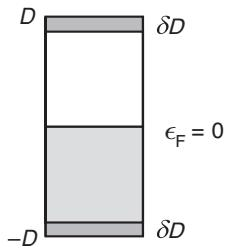
\includegraphics[width=0.42\textwidth]{figs/ch08/fig_8.7.jpg}
\caption*{图 8.7\quad 穷人标度法中要被消去的粒子态与空穴态。被移除的态的宽度为 $\delta D$。}\label{fig:auto:8.7}
\end{figure}

发展标度思想有许多途径，有简单的也有复杂的。我们将给出简单途径的一个精简版本 (H1993)。考虑一个满足 $-D < \epsilon_{\mathbf{k}} < D$ 的电子能带。如图 8.7 所示，我们的做法是分别从能带的下部和上部消去一窄层粒子态和空穴态，被消去态的宽度为 $\delta D$。基本想法是：考察进入二阶跃迁振幅的那些散射过程，确定当带宽缩减一个无穷小量 $\delta D$ 时它们如何变化。我们希望，随着带宽的缩减，能够找到一组把新的交换耦合与原有耦合联系起来的方程。

为简单起见，我们处理 $S=1/2$ 的杂质，但出于一般性的考虑，采用一个各向异性的自旋翻转哈密顿量
\begin{equation*}
H' = -\frac{1}{2\hbar V} \sum_{\mathbf{k}',\mathbf{k}'',\sigma} \Big[ J_{z} S_{d}^{z} \big( a_{\mathbf{k}'\uparrow}^{\dagger} a_{\mathbf{k}''\uparrow} - a_{\mathbf{k}'\downarrow}^{\dagger} a_{\mathbf{k}''\downarrow} \big) + J_{+} S_{d}^{+} a_{\mathbf{k}'\downarrow}^{\dagger} a_{\mathbf{k}''\uparrow} + J_{-} S_{d}^{-} a_{\mathbf{k}'\uparrow}^{\dagger} a_{\mathbf{k}''\downarrow} \Big],
\end{equation*}
其中自旋翻转部分（$J_{\pm}$）与纵向部分（$J_{z}$）具有不同的相互作用强度。我们的目标是化简二阶微扰项，证明它们导致 $J_{z}$ 与 $J_{\pm}$ 裸值的重正化。首先考虑图 8.8 所示的两个自旋翻转过程。由于双自旋翻转过程不改变杂质自旋，我们预期双自旋翻转项将导致纵向耦合 $J_{z}$ 的重正化。对 $J_{z}$ 修正的精确形式，可以对每一幅双自旋翻转图实施标度分析而得到。考虑第一幅图：
\begin{equation*}
J_{+}J_{-} \sum_{\mathbf{q}} \frac{S_{d}^{-}}{2\hbar V} a_{\mathbf{k}'\uparrow}^{\dagger} a_{\mathbf{q}\downarrow} \big( E - \widehat{H}_{0} \big)^{-1} \sum_{\mathbf{q}'} \frac{S_{d}^{+}}{2\hbar V} a_{\mathbf{q}'\downarrow}^{\dagger} a_{\mathbf{k}\uparrow}.
\tag{8.89}
\end{equation*}

\begin{figure}[H]\centering
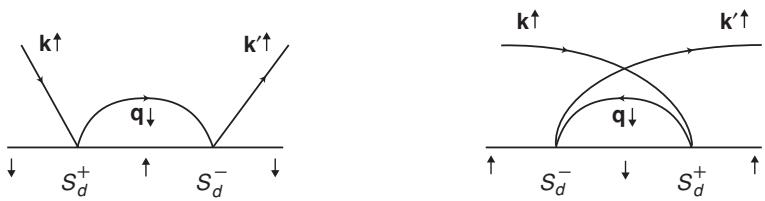
\includegraphics[width=0.72\textwidth]{figs/ch08/fig_8.8.jpg}
\caption*{图 8.8\quad 中间态包含粒子或空穴的二阶双自旋翻转图。实直线表示杂质自旋，曲线表示电子。}\label{fig:auto:8.8}
\end{figure}

为实施标度程序，我们把对 $\mathbf{q}'$ 的求和限制在距带顶 $\delta D$ 以内的状态，这些态由 $a_{\mathbf{q}'\downarrow}^{\dagger}$ 产生。由于带边态本来未被占据，必须取 $a_{\mathbf{q}} a_{\mathbf{q}'}^{\dagger} = \delta_{\mathbf{q},\mathbf{q}'}$。

在化简式 (8.89) 时，不能随意把最右边的产生和湮灭算符移过算符 $1/(E-\widehat{H}_{0})$，因为它们与 $\widehat{H}_{0}$ 不对易。对任一满足 $[\widehat{H}_{0}, \widehat{A}] = b\widehat{A}$ 的算符 $\widehat{A}$（其中 $b$ 是一个 c 数（c-number）），有 $\widehat{H}_{0}^{\,n}\widehat{A} = \widehat{A}(b + \widehat{H}_{0})^{n}$。于是
\begin{align*}
\frac{1}{E-\widehat{H}_{0}}\,\widehat{A} &= \frac{\widehat{A}}{E} \sum_{n=0}^{\infty} \frac{(\widehat{H}_{0}+b)^{n}}{E^{n}} \tag{8.90}\\
&= \widehat{A}\,\frac{1}{E-b-\widehat{H}_{0}}. \tag{8.91}
\end{align*}
利用 $[\widehat{H}_{0}, a_{\mathbf{q}'\downarrow}^{\dagger} a_{\mathbf{k}\uparrow}] = a_{\mathbf{q}'\downarrow}^{\dagger} a_{\mathbf{k}\uparrow} (\epsilon_{\mathbf{q}'} - \epsilon_{\mathbf{k}})$ 这一事实，我们把式 (8.89) 中的矩阵元化简为
\begin{equation*}
J_{+}J_{-} N(0)|\delta D| \frac{S_{d}^{-}S_{d}^{+}}{4V\hbar^{2}} a_{\mathbf{k}'\uparrow}^{\dagger} a_{\mathbf{k}\uparrow} \big( E - \epsilon_{\mathbf{q}} + \epsilon_{\mathbf{k}} - \widehat{H}_{0} \big)^{-1}.
\tag{8.92}
\end{equation*}
由于出现了 $a_{\mathbf{k}'\uparrow}^{\dagger} a_{\mathbf{k}\uparrow}$ 型的依赖，可以清楚地看到，双自旋翻转项改变了裸横向交换相互作用的取值。为提取精确的系数，我们利用 $S_{d}^{-}S_{d}^{+} = \hbar^{2}/2 - \hbar S_{d}^{z}$ 并取 $\epsilon_{\mathbf{q}} = D$。此外，若从带底量度 $E$，则可以忽略式 (8.92) 分母中 $\widehat{H}_{0}$ 的依赖。矩阵元化简为
\begin{equation*}
J_{+}J_{-} N(0) \frac{|\delta D|}{4\hbar V} \left( \frac{\hbar}{2} - S_{d}^{z} \right) a_{\mathbf{k}'\uparrow}^{\dagger} a_{\mathbf{k}\uparrow} \big( E - D + \epsilon_{\mathbf{k}} \big)^{-1}.
\tag{8.93}
\end{equation*}
现在可以用同样的方式计算图 8.8 中的第二幅图。这里中间态是粒子态，因此取 $\epsilon_{\mathbf{q}} = -D$，得到
\begin{equation*}
J_{+}J_{-} N(0) \frac{|\delta D|}{4\hbar V} \left( \frac{\hbar}{2} + S_{d}^{z} \right) a_{\mathbf{k}\uparrow} a_{\mathbf{k}'\uparrow}^{\dagger} \big( E - D - \epsilon_{\mathbf{k}'} \big)^{-1}.
\tag{8.94}
\end{equation*}
在推导此结果时，我们利用了关系式 $S_{d}^{+}S_{d}^{-} = \hbar^{2}/2 + \hbar S_{d}^{z}$。

其余涉及双自旋翻转的标度方程，可以通过计入来自 $\mathbf{k}\downarrow$ 与 $\mathbf{k}'\downarrow$ 的贡献得到。自旋向下状态之间的散射会产生正比于 $a_{\mathbf{k}\downarrow} a_{\mathbf{k}'\downarrow}^{\dagger}$ 的矩阵元，这一项将对 $S_{z}$ 算符的 $m_{s} = -1$ 自旋分量有贡献。

\begin{figure}[H]\centering
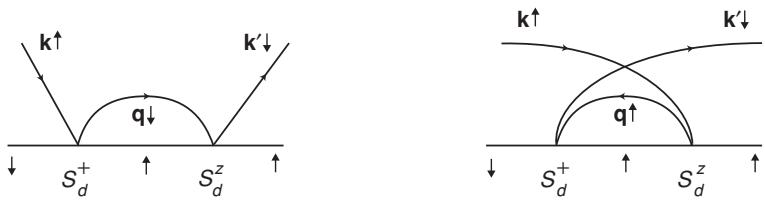
\includegraphics[width=0.72\textwidth]{figs/ch08/fig_8.9.jpg}
\caption*{图 8.9\quad 中间态包含粒子或空穴的二阶单自旋翻转图。实直线表示杂质自旋，曲线表示电子。}\label{fig:auto:8.9}
\end{figure}

现在定义新的纵向相互作用 $J_{z} \to J_{z} + \delta J_{z}$。注意到式 (8.89) 中裸相互作用的系数为 $1/2\hbar V$，我们发现式 (8.93) 与式 (8.94) 再结合自旋向下的方程，给出
\begin{equation*}
\delta J_{z} = \frac{1}{2} J_{+}J_{-} N(0)|\delta D| \left[ \frac{1}{E-D+\epsilon_{\mathbf{k}}} + \frac{1}{E-D-\epsilon_{\mathbf{k}'}} \right]
\tag{8.95}
\end{equation*}
作为对 $J_{z}$ 的修正。$J_{z}$ 的重正化依赖于能量。现在考虑能量远低于 $D$ 的激发，并在费米能级 $\epsilon_{\mathrm{F}} = 0$ 处取 $\epsilon_{\mathbf{k}}$ 与 $\epsilon_{\mathbf{k}'}$ 的值，$J_{z}$ 的标度方程便简化为
\begin{equation*}
\frac{\mathrm{d}J_{z}}{\mathrm{d}\ln D} = N(0)J_{\pm}^{2},
\tag{8.96}
\end{equation*}
其中我们已取 $\delta D$ 为负，并令 $J_{+} = J_{-} = J_{\pm}$。

现在考虑图 8.9 所示的单自旋翻转项。第一幅图的形式为
\begin{equation*}
- J_{+}J_{z} \sum_{\mathbf{q}} \frac{S_{d}^{z}}{2\hbar V} a_{\mathbf{k}'\downarrow}^{\dagger} a_{\mathbf{q}\downarrow} \big( E - \widehat{H}_{0} \big)^{-1} \sum_{\mathbf{q}'} \frac{S_{d}^{+}}{2\hbar V} a_{\mathbf{q}'\downarrow}^{\dagger} a_{\mathbf{k}'\uparrow}.
\tag{8.97}
\end{equation*}
该式前端的负号来源于 $S_{d}^{z}$ 的自旋向下分量所带的负号。用与双自旋翻转情形相同的技术，我们把该矩阵元化为
\begin{equation*}
\frac{- J_{+}J_{z} N(0)|\delta D| S_{d}^{+} a_{\mathbf{k}'\downarrow}^{\dagger} a_{\mathbf{k}\uparrow}}{8\hbar V \big( E - D + \epsilon_{\mathbf{k}} \big)},
\tag{8.98}
\end{equation*}
其中用到了 $S_{d}^{z}S_{d}^{+} = \hbar S_{d}^{+}/2$ 这一事实。因此，自旋翻转相互作用的重正化涉及 $J$ 的纵向分量。类似地，图 8.9 中另一幅图的取值为
\begin{equation*}
\frac{J_{+}J_{z} N(0)|\delta D| S_{d}^{+} a_{\mathbf{k}\uparrow} a_{\mathbf{k}'\downarrow}^{\dagger}}{8\hbar V \big( E - D - \epsilon_{\mathbf{k}'} \big)}.
\tag{8.99}
\end{equation*}
交换 $S_{d}^{z}$ 与 $S_{d}^{+}$ 的先后次序，可以得到这一形式的更多贡献，此时应使用恒等式 $S_{d}^{+}S_{d}^{z} = -\hbar S_{d}^{+}/2$。这里的贡献与式 (8.98) 和式 (8.99) 中的完全相同。

类似地，我们把单自旋翻转的结果与自旋向下电子散射的结果结合起来。定义新的横向相互作用 $J_{\pm}/2 \to (J_{\pm} + \delta J_{\pm})/2$，并利用式 (8.98) 与式 (8.99) 的结果，便得到交换相互作用横向分量的标度方程
\begin{equation*}
\delta J_{\pm} = \frac{1}{2} J_{\pm}J_{z} N(0)|\delta D| \left[ \frac{1}{E-D+\epsilon_{\mathbf{k}}} + \frac{1}{E-D-\epsilon_{\mathbf{k}'}} \right]
\tag{8.100}
\end{equation*}
这里同样地，横向耦合常数的标度依赖于能量。与纵向情形一样，我们考虑能量远低于 $D$ 的激发，并在费米能级 $\epsilon_{\mathrm{F}} = 0$ 处取 $\epsilon_{\mathbf{k}}$ 与 $\epsilon_{\mathbf{k}'}$ 的值，标度方程便简化为
\begin{equation*}
\frac{\mathrm{d}J_{\pm}}{\mathrm{d}\ln D} = N(0)J_{z}J_{\pm}.
\tag{8.101}
\end{equation*}

取式 (8.96) 与式 (8.101) 之比并积分，可以看到解是由
\begin{equation*}
J_{z}^{2} - J_{\pm}^{2} = \kappa,
\tag{8.102}
\end{equation*}
确定的一族双曲线，其中 $\kappa$ 为常数。为提取这些标度方程的物理结论，把式 (8.102) 代入 $J_{\pm}$ 的标度方程是有益的。对铁磁与反铁磁两种情形，我们发现
\begin{equation*}
\frac{\mathrm{d}J_{\pm}}{\mathrm{d}|\ln D|} =
\begin{cases}
-N(0)J_{\pm}\sqrt{\kappa + J_{\pm}^{2}}, & \quad J_{z} > 0, \quad \text{铁磁},\\
\phantom{-}N(0)J_{\pm}\sqrt{\kappa + J_{\pm}^{2}}, & \quad J_{z} < 0, \quad \text{反铁磁}.
\end{cases}
\tag{8.103}
\end{equation*}

标度分析的物理结论现在清楚了。由于式 (8.103) 的右端在 $J_{z} > 0$ 时为负，标度方程规定在此情形下 $J_{\pm} \to 0$。结果，在铁磁情形，横向交换耦合随带宽的缩减变得越来越弱。然而，在反铁磁情形，式 (8.103) 的右端为正，标度方程规定 $|J_{\pm}| \to \infty$。这就是发生近藤效应的强耦合区域。交换耦合的幅值随带宽的减小而增大。正是交换相互作用在带宽减小时被自举到更大的数值，导致了近藤杂质处单态的形成。

图 8.10 所示的流图使标度分析一目了然。双曲线是各向异性耦合（$|J_{+}| > |J_{z}|$）的结果，直线则是各向同性耦合极限下解坍缩为 $|J_{+}|^{2} = J_{z}^{2}$ 的情形。箭头指向 $D$ 减小的方向。$J_{z}$ 为正（铁磁耦合）的曲线表明，随着 $D$ 趋于零，$J_{z}$ 与 $|J_{+}|$ 流向零；而 $J_{z}$ 为负（反铁磁耦合）的曲线则表明，随着 $D$ 趋于零，两个耦合都发散。各向同性极限与各向异性极限展现出相同的物理。

\begin{figure}[H]\centering
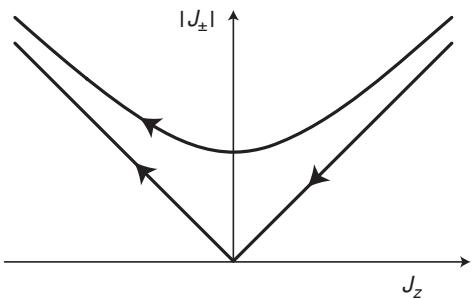
\includegraphics[width=0.5\textwidth]{figs/ch08/fig_8.10.jpg}
\caption*{图 8.10\quad 用 Anderson 的二阶微扰论论证得到的近藤模型标度轨迹。双曲线对应各向异性耦合，直线对应各向同性耦合。$J_{z} > 0$ 的区域对应铁磁耦合，$J_{z} < 0$ 的区域对应反铁磁耦合。}\label{fig:auto:8.10}
\end{figure}

在各向同性极限下，$J_{\pm}(D) = J_{z}(D) = J(D)$，标度方程约化为单一方程
\begin{equation*}
\frac{\mathrm{d}J}{\mathrm{d}\ln D} = J^{2}N(0),
\tag{8.104}
\end{equation*}
其解为
\begin{equation*}
J(D) = \frac{J(D_{0})}{1 - J(D_{0})N(0)\ln(D/D_{0})},
\tag{8.105}
\end{equation*}
其中 $D_{0}$ 是初始带宽。物理上，我们感兴趣的情形是：有效带宽处于有限温度下电子所能探及的状态范围，即费米面附近宽度为 $k_{\mathrm{B}}T$ 的区间。于是在对数精度下可以取 $D/D_{0} = k_{\mathrm{B}}T/\epsilon_{\mathrm{F}} = T/T_{\mathrm{F}}$。作了这一认定后，式 (8.105) 与式 (8.64) 完全等价。

下面从标度方程中提取近藤温度。这样做时，重要的是记住近藤温度是一个物理量，因而不应依赖于我们在模型描述中选取的带宽 $D$，也就是说，$T_{\mathrm{k}}$ 应当是标度不变的，
\begin{equation*}
D\frac{\partial T_{\mathrm{k}}}{\partial D} = 0.
\tag{8.106}
\end{equation*}
这样一来，所有物理量（如电阻率和磁化率）都将依赖于比值 $T/T_{\mathrm{k}}$（对 $T/T_{\mathrm{F}}$ 的依赖则奇异性较弱），而不依赖于 $D$。

如果我们在各向同性情形下定义无量纲耦合常数 $g = N(0)J$，标度方程便成为
\begin{equation*}
\frac{\mathrm{d}g}{\mathrm{d}\ln D} \equiv \beta(g) = g^{2}.
\tag{8.107}
\end{equation*}
耦合常数的对数导数通常称为 $\beta$ 函数，得名于盖尔曼（Gell-Mann）和洛（Low）(GL1954)；在第 13 章讨论局域化时我们还会遇到这个概念。从量纲上看，近藤温度必须具有 $k_{\mathrm{B}}T_{\mathrm{k}} = Dy(g)$ 的形式，其中 $D$ 确定能标。为确定 $y$，把 $T_{\mathrm{k}}$ 的这一形式代入标度不变条件，即式 (8.106)，得到线性微分方程
\begin{equation*}
y(g) + \frac{\partial y}{\partial g}\frac{\partial g}{\partial \ln D} = 0.
\tag{8.108}
\end{equation*}
其解很简单：
\begin{equation*}
y(g) \sim \mathrm{e}^{1/g}.
\tag{8.109}
\end{equation*}
因此，近藤温度由 $k_{\mathrm{B}}T_{\mathrm{k}} = D\exp(1/(N(0)J))$ 给出，与我们先前看到的式 (8.86) 的结构一致。近藤温度与带宽无关，而前面却又显含因子 $D$，这看似矛盾，其实不然。对 $D$ 的补偿性依赖藏在耦合常数 $g$ 之中，使得式 (8.106) 得以满足。

近藤问题的完整标度结构，由威尔逊（Wilson）在对该问题的关键性重正化群分析 (W1975) 中确定。威尔逊证明，随着能标趋于零，本征态的分布变得大致等价于 $J \to -\infty$ 的体系的分布。因此，初始具有小交换相互作用的体系，随着能标的降低，平滑地交叉过渡（crossover）到交换相互作用向负方向发散的体系。正是相互作用的发散导致了近藤问题中向单态基态的交叉过渡。不过，在威尔逊重正化群方法中，发散发生在 $T = 0$，而不是在有限的 $T_{\mathrm{k}}$ 处；这里 $T_{\mathrm{k}}$ 处的发散，是微扰论中领头对数（leading logarithm）求和造成的假象。

至此，关于近藤问题的故事大体讲完了。不过，更晚近的理论工作还包括：Nozières (N1974) 关于 $T_{\mathrm{k}}$ 以下费米液体图像的工作、Anderson 模型与近藤模型的精确贝特拟设（Bethe ansatz）解 (TW1983; AFL1983)，以及共形场论方法 (AL1991; AZ1996)。计入电子关联 (LT1992) 会使近藤温度随交换耦合按代数（幂律）方式而非指数方式标度，这与这里讨论的不同；其幂指数正比于导带电子之间相互作用的强度。此外，理论预言即使对铁磁相互作用，近藤单态也可以稳定存在 (FN1994)，这一结果是在卢廷格液体的框架内建立的，我们将在第 10 章讨论。

\section*{小结}
\addcontentsline{toc}{section}{小结}

低温下金属中局域磁矩的淬灭，正是近藤问题背后的物理。这一效应来源于钉扎在费米能级上的多体共振。本章我们着重于从相当简单的考虑出发提取这一图像。近藤温度是一个标度不变量，由 $T_{\mathrm{k}} = D\exp(1/g)$ 给出，其中 $g = N(0)J$ 是有效裸近藤交换相互作用。从微扰的角度看，近藤温度可以认定为这样的能标：在此能标处，微扰论中的二阶项变得与 $J$ 的线性项同量级——这是微扰论正在失效、高阶项同样重要的标志。费米能级处的共振是真正的多粒子效应：微扰论中的 $n$ 阶项包含 $n$ 个电子与局域磁矩的相互作用。正是对所有这些项的求和产生了共振。

\section*{本章附录：Schrieffer--Wolff 变换}
\addcontentsline{toc}{section}{本章附录：Schrieffer--Wolff 变换}

在本附录中，我们从 Anderson 哈密顿量出发，完整地推导近藤哈密顿量中的交换相互作用。由于 Anderson 哈密顿量既包含空的也包含双占据的杂质态，一个生成近藤哈密顿量的变换，等价于把 Anderson 哈密顿量在单占据杂质态的子空间内对角化。这一对角化由 Schrieffer--Wolff 变换 (SW1966) 完成。

我们先把 Anderson 哈密顿量分解为零阶部分
\begin{equation*}
H_{0} = \sum_{\mathbf{k},\sigma} \epsilon_{\mathbf{k}} n_{\mathbf{k}\sigma} + \epsilon_{d} \sum_{\sigma} n_{d\sigma} + U n_{d\uparrow} n_{d\downarrow}
\tag{8.110}
\end{equation*}
和微扰部分
\begin{equation*}
H_{1} = \sum_{\mathbf{k}\sigma} V_{\mathbf{k}d} \big( a_{\mathbf{k}\sigma}^{\dagger} a_{d\sigma} + a_{d\sigma}^{\dagger} a_{\mathbf{k}\sigma} \big).
\tag{8.111}
\end{equation*}
在本推导中，取 $V_{\mathbf{k}d}$ 为实数。

为推进推导，我们对原哈密顿量施行一个正则变换（或相似变换）$S$：
\begin{equation*}
\begin{aligned}
\widetilde{H} &= \mathrm{e}^{S} H \mathrm{e}^{-S} \\
&= H + [S, H] + \frac{1}{2}[S, [S, H]] + \cdots.
\end{aligned}
\end{equation*}
注意，由于 $\mathrm{e}^{S}$ 是幺正的，$S$ 必须是反厄米的。如果选取 $S$ 使之消去对微扰 $H_{1}$ 的线性依赖，即
\begin{equation*}
H_{1} + [S, H_{0}] = 0
\tag{8.112}
\end{equation*}
那么精确到最低阶的新哈密顿量为
\begin{equation*}
\widetilde{H} = H_{0} + \frac{1}{2}[S, H_{1}],
\tag{8.113}
\end{equation*}
从而把电荷涨落纳入到 $V_{\mathbf{k}d}$ 的二阶。一旦辨识出小量，相似变换方法就是进行微扰分析的一种一般方法。

$S$ 的显式形式可以这样构造：注意到由于 $[S, H_{0}] = -H_{1}$，算符 $S$ 必须含有正比于 $a_{\mathbf{k}\sigma}^{\dagger} a_{d\sigma}$ 的项；此外，它与 $U n_{d\uparrow} n_{d\downarrow}$ 的对易子给出正比于 $n_{d-\sigma} a_{\mathbf{k}\sigma}^{\dagger} a_{d\sigma}$ 的项。这提示我们尝试如下形式的变换
\begin{equation*}
S = \sum_{\mathbf{k},\sigma} \big( A_{\mathbf{k}} + B_{\mathbf{k}} n_{d-\sigma} \big) a_{\mathbf{k}\sigma}^{\dagger} a_{d\sigma} - \mathrm{h.c.},
\tag{8.114}
\end{equation*}
其中 $A_{\mathbf{k}}$ 与 $B_{\mathbf{k}}$ 是有待由式 (8.112) 确定的 c 数。

利用如下对易关系：
\begin{equation*}
\begin{aligned}
& \big[ n_{d\sigma}, a_{d\sigma'} \big] = -\delta_{\sigma\sigma'} a_{d\sigma}, \\
& \big[ n_{d\sigma}, n_{d\sigma'} \big] = 0, \\
& \big[ n_{d\sigma} n_{d-\sigma}, a_{d\sigma'} \big] = -\delta_{\sigma\sigma'} n_{d-\sigma} a_{d\sigma} - \delta_{-\sigma\sigma'} n_{d\sigma} a_{d\sigma'},
\end{aligned}
\tag{8.115}
\end{equation*}
再加上关系式 $[A, B^{\dagger}] = -[A, B]^{\dagger}$（当 $A = A^{\dagger}$ 时成立），我们直接计算 $H_{0}$ 与 $S$ 的对易子，得到
\begin{align*}
[H_{0}, S] = {} & \sum_{\mathbf{k},\sigma} \epsilon_{\mathbf{k}} \big( A_{\mathbf{k}} + B_{\mathbf{k}} n_{d-\sigma} \big) a_{\mathbf{k}\sigma}^{\dagger} a_{d\sigma} + \mathrm{h.c.} + \sum_{\mathbf{k},\sigma} \epsilon_{d} \big( -A_{\mathbf{k}} - B_{\mathbf{k}} n_{d-\sigma} \big) a_{\mathbf{k}\sigma}^{\dagger} a_{d\sigma} + \mathrm{h.c.} \\
& + U \sum_{\mathbf{k},\sigma} \big( -A_{\mathbf{k}} n_{d-\sigma} - B_{\mathbf{k}} n_{d-\sigma} \big) a_{\mathbf{k}\sigma}^{\dagger} a_{d\sigma} + \mathrm{h.c.} \\
= {} & \sum_{\mathbf{k},\sigma} \big[ (\epsilon_{\mathbf{k}} - \epsilon_{d}) A_{\mathbf{k}} + (\epsilon_{\mathbf{k}} - \epsilon_{d} - U) n_{d-\sigma} B_{\mathbf{k}} - A_{\mathbf{k}} U n_{d-\sigma} \big] a_{\mathbf{k}\sigma}^{\dagger} a_{d\sigma} + \mathrm{h.c.}, \tag{8.116}
\end{align*}
其中 h.c. 表示厄米共轭。为满足式 (8.112)，我们要求 $(\epsilon_{\mathbf{k}} - \epsilon_{d}) A_{\mathbf{k}} = V_{\mathbf{k}d}$ 以及 $(\epsilon_{\mathbf{k}} - \epsilon_{d} - U) B_{\mathbf{k}} - A_{\mathbf{k}} U = 0$，于是
\begin{equation*}
A_{\mathbf{k}} = \frac{V_{\mathbf{k}d}}{\epsilon_{\mathbf{k}} - \epsilon_{d}}
\end{equation*}
且
\begin{equation*}
B_{\mathbf{k}} = V_{\mathbf{k}d} \left[ \frac{1}{\epsilon_{\mathbf{k}} - (\epsilon_{d} + U)} - \frac{1}{\epsilon_{\mathbf{k}} - \epsilon_{d}} \right].
\end{equation*}
式 (8.114) 连同常数 $A_{\mathbf{k}}$、$B_{\mathbf{k}}$ 的这组定义，就完全确定了 Schrieffer--Wolff 变换。

为求新哈密顿量，需要计算对易子 $[S, H_{1}]$：
\begin{align*}
[S, H_{1}] = \sum_{\mathbf{k},\sigma,\mathbf{k}',\sigma'} \big\{ {} & A_{\mathbf{k}} V_{\mathbf{k}'d} \big[ \rho_{\mathbf{k}d\sigma}, \big( \rho_{\mathbf{k}'d\sigma'} + \rho_{\mathbf{k}'d\sigma'}^{\dagger} \big) \big] - B_{\mathbf{k}}^{*} V_{\mathbf{k}'d} \big[ n_{d-\sigma} \rho_{\mathbf{k}d\sigma}^{\dagger}, \big( \rho_{\mathbf{k}'d\sigma'} + \rho_{\mathbf{k}'d\sigma'}^{\dagger} \big) \big] \\
& + B_{\mathbf{k}} V_{\mathbf{k}'d} \big[ n_{d-\sigma} \rho_{\mathbf{k}d\sigma}, \big( \rho_{\mathbf{k}'d\sigma'} + \rho_{\mathbf{k}'d\sigma'}^{\dagger} \big) \big] - A_{\mathbf{k}}^{*} V_{\mathbf{k}'d} \big[ \rho_{\mathbf{k}d\sigma}^{\dagger}, \big( \rho_{\mathbf{k}'d\sigma'} + \rho_{\mathbf{k}'\sigma'}^{\dagger} \big) \big] \big\}, \tag{8.117}
\end{align*}
这里通过定义 $\rho_{\mathbf{k}d\sigma} = a_{\mathbf{k}\sigma}^{\dagger} a_{d\sigma}$ 简化了记号。在这一步，下列对易关系很有用：
\begin{equation*}
\begin{aligned}
& \big[ \rho_{\mathbf{k}d\sigma}, \rho_{\mathbf{k}'d\sigma'} \big] = 0, \\
& \big[ \rho_{\mathbf{k}d\sigma}, \rho_{\mathbf{k}'d\sigma'}^{\dagger} \big] = \delta_{\sigma\sigma'} \big[ -\delta_{\mathbf{k}\mathbf{k}'} n_{d\sigma} + a_{\mathbf{k}\sigma}^{\dagger} a_{\mathbf{k}'\sigma} \big], \\
& \big[ n_{d-\sigma} \rho_{\mathbf{k}d\sigma}, \rho_{\mathbf{k}'d\sigma'} \big] = -\delta_{\sigma'-\sigma} \rho_{\mathbf{k}d\sigma} \rho_{\mathbf{k}'d-\sigma}, \\
& \big[ n_{d-\sigma} \rho_{\mathbf{k}d\sigma}, \rho_{\mathbf{k}'d\sigma'}^{\dagger} \big] = \delta_{-\sigma\sigma'} \rho_{\mathbf{k}d\sigma} \rho_{\mathbf{k}'d-\sigma}^{\dagger} + \delta_{\sigma\sigma'} \big( a_{\mathbf{k}\sigma}^{\dagger} a_{\mathbf{k}'\sigma} n_{d-\sigma} - \delta_{\mathbf{k}\mathbf{k}'} n_{d-\sigma} n_{d\sigma} \big).
\end{aligned}
\end{equation*}
把这些关系代入式 (8.117)，得到
\begin{align*}
[S, H_{1}] = {} & -\sum_{\mathbf{k},\sigma} \big( A_{\mathbf{k}} V_{\mathbf{k}d} + B_{\mathbf{k}} V_{\mathbf{k}d} n_{d-\sigma} \big) n_{d\sigma} + \mathrm{h.c.} + \sum_{\mathbf{k},\mathbf{k}',\sigma} A_{\mathbf{k}} V_{\mathbf{k}'d} a_{\mathbf{k}\sigma}^{\dagger} a_{\mathbf{k}'\sigma} + \mathrm{h.c.} \\
& -\sum_{\mathbf{k},\mathbf{k}',\sigma} B_{\mathbf{k}} V_{\mathbf{k}'d} \rho_{\mathbf{k}\sigma} \rho_{\mathbf{k}'-\sigma} + \mathrm{h.c.} + \sum_{\mathbf{k},\mathbf{k}',\sigma} B_{\mathbf{k}} V_{\mathbf{k}'d} \big[ a_{\mathbf{k}\sigma}^{\dagger} a_{\mathbf{k}'\sigma} n_{d-\sigma} + \rho_{\mathbf{k}\sigma} \rho_{\mathbf{k}'-\sigma}^{\dagger} \big] + \mathrm{h.c.} \tag{8.118}
\end{align*}

把最后一项中的算符写成
\begin{equation*}
\begin{aligned}
& \big[ a_{\mathbf{k}\sigma}^{\dagger} a_{\mathbf{k}'\sigma} n_{d-\sigma} + \rho_{\mathbf{k}d\sigma} \rho_{\mathbf{k}'d-\sigma}^{\dagger} \big] = \frac{1}{2} \big( n_{d\sigma} + n_{d-\sigma} \big) a_{\mathbf{k}\sigma}^{\dagger} a_{\mathbf{k}'\sigma} \\
& \qquad - \frac{1}{2} \big[ \big( n_{d\sigma} - n_{d-\sigma} \big) a_{\mathbf{k}\sigma}^{\dagger} a_{\mathbf{k}'\sigma} - 2 \rho_{\mathbf{k}d\sigma} \rho_{\mathbf{k}'d-\sigma}^{\dagger} \big].
\end{aligned}
\tag{8.119}
\end{equation*}
这一项的第二部分给出近藤交换相互作用。为看出这一点，注意到乘积
\begin{align*}
\frac{4}{\hbar^{2}} \big( \Psi_{\mathbf{k}'}^{\dagger} \mathbf{S} \Psi_{\mathbf{k}} \big) \cdot \big( \Psi_{d}^{\dagger} \mathbf{S} \Psi_{d} \big) ={} & \big( \Psi_{\mathbf{k}'}^{\dagger} \sigma_{z} \Psi_{\mathbf{k}} \big) \cdot \big( \Psi_{d}^{\dagger} \sigma_{z} \Psi_{d} \big) + 2 \big( \Psi_{\mathbf{k}'}^{\dagger} \sigma^{+} \Psi_{\mathbf{k}} \big) \big( \Psi_{d}^{\dagger} \sigma^{-} \Psi_{d} \big) \\
& + 2 \big( \Psi_{\mathbf{k}'}^{\dagger} \sigma^{-} \Psi_{\mathbf{k}} \big) \big( \Psi_{d}^{\dagger} \sigma^{+} \Psi_{d} \big) \\
={}& \sum_{\sigma} \big[ a_{\mathbf{k}'\sigma}^{\dagger} a_{\mathbf{k}\sigma} \big( n_{d\sigma} - n_{d-\sigma} \big) - 2 \rho_{\mathbf{k}'d\sigma} \rho_{\mathbf{k}d-\sigma}^{\dagger} \big] \tag{8.120}
\end{align*}
恰好具有式 (8.119) 最后一项的形式。对 $\widetilde{H}$ 的相应贡献是
\begin{equation*}
H_{\mathrm{exch}} = -\frac{1}{\hbar^{2}} \sum_{\mathbf{k},\mathbf{k}'} J_{\mathbf{k}\mathbf{k}'} \big( \Psi_{\mathbf{k}'}^{\dagger} \mathbf{S} \Psi_{\mathbf{k}} \big) \cdot \big( \Psi_{d}^{\dagger} \mathbf{S} \Psi_{d} \big),
\tag{8.121}
\end{equation*}
其中
\begin{equation*}
\begin{aligned}
J_{\mathbf{k}\mathbf{k}'} &= \big( B_{\mathbf{k}'} V_{\mathbf{k}d} + B_{\mathbf{k}}^{*} V_{\mathbf{k}'d} \big) \\
&= V_{\mathbf{k}'d} V_{\mathbf{k}d} \left[ \frac{1}{\epsilon_{\mathbf{k}'} - (\epsilon_{d} + U)} + \frac{1}{\epsilon_{\mathbf{k}} - (\epsilon_{d} + U)} - \frac{1}{\epsilon_{\mathbf{k}} - \epsilon_{d}} - \frac{1}{\epsilon_{\mathbf{k}'} - \epsilon_{d}} \right].
\end{aligned}
\tag{8.122}
\end{equation*}

这一项来源于式 (8.119) 的最后一项，它就是近藤相互作用。注意，这个结果就是由二阶微扰论导出的式 (8.10) 的形式，只是对 $\mathbf{k}$ 与 $\mathbf{k}'$ 对称化了。我们在这里看到了相似变换方法的一个特别优点：即使初末态能量不同，它也能正确地给出相互作用矩阵元。相比之下，只有当初末态具有相同能量时，我们才能把二阶散射振幅与相互作用矩阵元等同起来，此时式 (8.10) 与式 (8.122) 一致。在费米能级附近，$k, k' \sim k_{\mathrm{F}}$，自旋交换振幅约化为
\begin{equation*}
J_{k_{\mathrm{F}} k_{\mathrm{F}}} \equiv J_{0} = -2 V_{\mathbf{k}d}^{2} \frac{U}{|\epsilon_{d}| (U - |\epsilon_{d}|)} < 0,
\tag{8.123}
\end{equation*}
一如前述。（译注：原书此式分母印作 $(|\epsilon_{d}| - U)$，如此则式值为正，与其后的“$<0$”矛盾；按式 (8.11) 应为 $(U - |\epsilon_{d}|)$，译文已据此改正。原书此处耦合常数下标又印作 $J_{o}$，为与全章一致，统一记作 $J_{0}$。）

总起来，可以把 $\widetilde{H}$ 写成
\begin{equation*}
\begin{aligned}
\widetilde{H} &= H_{0} + \frac{1}{2}[S, H_{1}] \\
&= H_{0} + H_{0}' + H_{0}'' + H_{\mathrm{exch}} + H_{\mathrm{dir}} + H_{\mathrm{ch}}.
\end{aligned}
\tag{8.124}
\end{equation*}
直接项
\begin{equation*}
H_{\mathrm{dir}} = \sum_{\mathbf{k},\mathbf{k}'} \frac{1}{4} J_{\mathbf{k}\mathbf{k}'} \big( \Psi_{d}^{\dagger} \Psi_{d} \big) \big( \Psi_{\mathbf{k}'}^{\dagger} \Psi_{\mathbf{k}} \big)
\tag{8.125}
\end{equation*}
来源于式 (8.119) 的第一项。这里
\begin{equation*}
\begin{aligned}
W_{\mathbf{k}\mathbf{k}'} &= \frac{1}{2} \big( A_{\mathbf{k}'} V_{\mathbf{k}d} + A_{\mathbf{k}}^{*} V_{\mathbf{k}'d} \big) \\
&= \frac{1}{2} V_{\mathbf{k}'d} V_{\mathbf{k}d} \left[ \frac{1}{\epsilon_{\mathbf{k}'} - \epsilon_{d}} + \frac{1}{\epsilon_{\mathbf{k}} - \epsilon_{d}} \right].
\end{aligned}
\tag{8.126}
\end{equation*}
$W_{\mathbf{k}\mathbf{k}'}$ 中出现的能量分母，只涉及如图 8.2(b) 所示的、只及杂质上最低态的激发过程，而 $J_{\mathbf{k}\mathbf{k}'}$ 则包含图 8.2 中的两个过程。由于 $J_{\mathbf{k}\mathbf{k}'}$ 与 $W_{\mathbf{k}'\mathbf{k}}$ 来自相继的激发和退激发过程，在它们所描述的过程中杂质保持单占据。

项
\begin{equation*}
H_{0}' = -\sum_{\mathbf{k}\sigma} \left( W_{\mathbf{k}\mathbf{k}} + \frac{1}{2} J_{\mathbf{k}\mathbf{k}} n_{d-\sigma} \right) n_{d\sigma},
\tag{8.127}
\end{equation*}
由式 (8.118) 的第一项给出。类似地，项
\begin{equation*}
H_{0}'' = \sum_{\mathbf{k},\mathbf{k}'} W_{\mathbf{k}\mathbf{k}'} \Psi_{\mathbf{k}}^{\dagger} \Psi_{\mathbf{k}'},
\tag{8.128}
\end{equation*}
来源于式 (8.119) 的第二项，它表示单个电子所感受到的势的重正化。$H_{0}'$ 与 $H_{0}''$ 都对理解近藤问题很重要，因为它们进入非自旋翻转的过程。

\begin{figure}[H]\centering
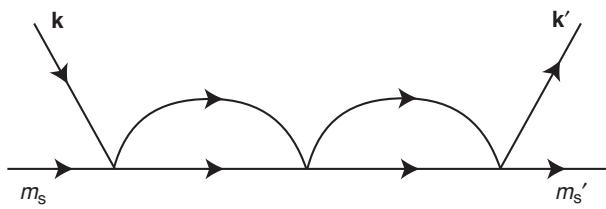
\includegraphics[width=0.6\textwidth]{figs/ch08/fig_8.11.jpg}
\caption*{图 8.11\quad 对标度给出线性修正的三阶近藤图（见习题 8.4）。}\label{fig:auto:8.11}
\end{figure}

最后一项
\begin{equation*}
H_{\mathrm{ch}} = -\frac{1}{2} \sum_{\mathbf{k},\mathbf{k}',\sigma} \big( B_{\mathbf{k}} V_{\mathbf{k}'d} \rho_{\mathbf{k}\sigma} \rho_{\mathbf{k}'-\sigma} + \mathrm{h.c.} \big),
\tag{8.129}
\end{equation*}
来源于式 (8.118) 的第三项，它使 d 杂质的占据数改变 2，因此对近藤问题同样不重要。相互作用中两个重要的项，是自旋交换过程和直接的杂质--电子散射项。

让我们把对应于杂质单占据的项分离出来。首先注意到，由于 $H_{\mathrm{ch}}$ 把 d 杂质上的两个电子都移走，它无法与希尔伯特空间中的单电子态相联系，我们舍去这一项。此外，在单电子子空间中 $\Psi_{d}^{\dagger} \Psi_{d} = 1$。因此，$H_{\mathrm{dir}}$ 是一个单电子项，$H_{0}'$ 与 $H_{0}''$ 也是。在这个子空间中，$H_{\mathrm{exch}}$ 是唯一重要的项。准确到 $V_{\mathbf{k}d}$ 的二阶，Anderson 模型给出具有反铁磁交换耦合的近藤模型。正是这一相互作用的反铁磁性质，导致了 d 杂质处向单态的凝聚。

\section*{习题}
\addcontentsline{toc}{section}{习题}

\textbf{习题 8.1}\quad (a) 大小固定的磁矩，其能量在磁场中是线性的。证明：这种磁矩的无相互作用集合的高温（居里）磁化率与 $T$ 成反比。

(b) 另一方面，可极化单态的能量在磁场中是二次的。证明：这种磁矩的无相互作用集合的磁化率在低温下趋于常数。

\textbf{习题 8.2}\quad 在杂质与导带电子之间存在铁磁自旋--自旋相互作用的情形下，重复 Yosida 的单电子变分计算，导出一个三重态束缚态。求解相应的三重态稳定性方程，并计算三重态的结合能。与单态相比，在相同的 $|J_{0}|$ 下哪一个能量更低？

\textbf{习题 8.3}\quad 求解各向异性标度方程（解析地或数值地），并验证它们满足图 8.10 所示的流图。

\textbf{习题 8.4}\quad 考虑图 8.11 所示的三阶近藤图。解释这幅图如何能给出一个线性于 $\delta D$ 的标度修正。假定 $\mathbf{q}$ 与 $\mathbf{q}'$ 相互独立。显式地计算标度系数。

\textbf{习题 8.5}\quad 利用由 Schrieffer--Wolff 变换导出的完整哈密顿量，即式 (8.124)，计算最低阶散射振幅：$T[(\mathbf{k}\sigma)+(d-\sigma) \to (\mathbf{k}'\sigma)+(d-\sigma)]$、$T[(\mathbf{k}\sigma)+(d\sigma) \to (\mathbf{k}'\sigma)+(d\sigma)]$ 与 $T[(\mathbf{k}\sigma)+(d-\sigma) \to (\mathbf{k}'-\sigma)+(d\sigma)]$，并与 8.2 节给出的结果比较。

\section*{参考文献}
\addcontentsline{toc}{section}{参考文献}

\begin{itemize}[leftmargin=2em,itemsep=0pt,parsep=0pt,label={}]
\item {[A1957]} A. A. Abrikosov, \emph{Physics} \textbf{2}, 5 (1965).
\item {[AL1991]} I. Affleck and A. W. W. Ludwig, \emph{Nucl. Phys. B} \textbf{352}, 849 (1991).
\item {[A1964]} P. W. Anderson, \emph{Phys. Rev.} \textbf{124}, 41 (1961).
\item {[AYH1970]} P. W. Anderson, G. Yuval, and D. R. Hamann, \emph{Phys. Rev. B} \textbf{1}, 4464 (1970).
\item {[A1978]} P. W. Anderson, \emph{Rev. Mod. Phys.} \textbf{50}, 191 (1978).
\item {[AFL1983]} N. Andrei, K. Furuya, and J. H. Lowenstein, \emph{Rev. Mod. Phys.} \textbf{55}, 331 (1983).
\item {[AZ1996]} V. Barzykin and I. Affleck, \emph{Phys. Rev. Lett.} \textbf{76}, 4959 (1996).
\item {[FN1994]} A. Furusaki and N. Nagaosa, \emph{Phys. Rev. Lett.} \textbf{72}, 892 (1994).
\item {[GL1954]} M. Gell-Mann and F. Low, \emph{Phys. Rev.} \textbf{111}, 582 (1954).
\item {[GZ1972]} G. Gr\"{u}ner and A. Zawadowski, \emph{Solid St. Comm.} \textbf{11}, 663 (1972).
\item {[H1969]} A. J. Heeger, in \emph{Solid State Physics}, eds. F. Seitz, D. Turnbull, and H. Ehrenreich (Academic Press, New York, 1969), p.~283.
\item {[H1993]} A. C. Hewson, \emph{The Kondo Problem to Heavy Fermions} (Cambridge University Press, New York, 1993).
\item {[K1956]} T. Kasuya, \emph{Prog. Theor. Phys.} \textbf{16}, 45 (1956).
\item {[K1964]} J. Kondo, \emph{Prog. Theor. Phys.} \textbf{32}, 37 (1964).
\item {[L1981]} C. Lacroix, \emph{J. Phys. F: Metal Phys.} \textbf{11}, 2389 (1981).
\item {[LT1992]} D. H. Lee and J. Toner, \emph{Phys. Rev. Lett.} \textbf{72}, 892 (1992).
\item {[N1974]} P. Nozi\`{e}res, \emph{J. Low Temp. Phys.} \textbf{17}, 31 (1974).
\item {[SCL1964]} M. Sarachik, E. Corenzwit, and L. D. Longinotti, \emph{Phys. Rev. A} \textbf{135}, 1041 (1964).
\item {[SW1966]} J. R. Schrieffer and P. A. Wolff, \emph{Phys. Rev.} \textbf{149}, 491 (1966).
\item {[SZ1974]} J. Solyom and A. Zawadowski, \emph{J. Phys. F: Metal Phys.} \textbf{4}, 80 (1974).
\item {[TW1983]} A. M. Tsvelick and P. B. Wiegmann, \emph{Adv. in Phys.} \textbf{32}, 453 (1983).
\item {[V1946]} S. Vousovskii, \emph{Zh. Eksp. Teor. Fiz.} \textbf{16}, 981 (1946).
\item {[W1975]} K. Wilson, \emph{Rev. Mod. Phys.} \textbf{47}, 773 (1975).
\item {[Y1966]} K. Yosida, \emph{Phys. Rev.} \textbf{147}, 223 (1966).
\item {[Z1951]} C. Zener, \emph{Phys. Rev.} \textbf{81}, 440 (1951).
\end{itemize}
